\documentclass[12pt]{article}
%\usepackage[utf8]{inputenc}
\usepackage[french]{babel} 
\usepackage[T1]{fontenc}
\usepackage{graphicx}
\usepackage{xcolor}
\usepackage{lmodern}
\usepackage{array}
\usepackage{float}
\usepackage{listings}

%load default definitions 
%%novalidate

\usepackage{tikz}
\usepackage{calc}
\usepackage{booktabs}
%\usepackage{hyperref}

% colors
\definecolor{color1}{HTML}{000060}
%\definecolor{color1}{HTML}{8C260F}
\definecolor{color2}{HTML}{333333}


% fonts
\usepackage{fontspec}
\defaultfontfeatures{Mapping=tex-text}
\setmainfont
[BoldFont=Lato-Bold.ttf,
ItalicFont=Lato-Italic.ttf,
BoldItalicFont=Lato-BoldItalic.ttf]
{Lato-Regular.ttf}
\newfontfamily\headingfont[ItalicFont=Lato-BlackItalic.ttf]{Lato-Black.ttf}
%%%

\usepackage{geometry}
\geometry{a4paper,
hmargin=20mm,vmargin=20mm,
head=15pt,foot=3ex}

\linespread{1.3}

\usepackage[hang]{caption}
\DeclareCaptionFormat{upper}{#1#2\uppercase{#3}\par}
\captionsetup{labelfont={bf,color=color2},textfont={normalsize,color=color2},format = upper,figurename=FIGURE,tablename=TABLE}

%%% fancy sections
\usepackage{titlesec}
%\titleformat{\chapter}{\headingfont\LARGE\bfseries\scshape\color{color1}}{\thechapter}{1em}{}[\titlerule]
\titleformat{\section}{\color{color1}\headingfont\Large\bfseries\uppercase}{\thesection}{1em}{}[\titlerule]
\titleformat{\subsection}{\color{color1}\headingfont\large\bfseries\uppercase}{\thesubsection}{1em}{}
\titleformat{\subsubsection}{\color{color1}\headingfont\bfseries\uppercase}{\thesubsubsection}{1em}{}
%%%

% head and foot
\usepackage{fancyhdr}
\pagestyle{fancy}
\lhead{}
\chead{}
\makeatletter
\rhead{\color{color2}\@date}
\makeatother
\newlength{\myheight}
\lfoot{
\settoheight{\myheight}{\thepage}
\raisebox{-2ex-0.5\myheight}{
\includegraphics[height=4ex]{logo}}
}
\cfoot{\color{color2} Projet adenome-pro 2017/2018 }
\rfoot{\color{color2}\thepage}
\renewcommand\headrulewidth{0pt}
\renewcommand\footrulewidth{0pt}

%%% picture on cover page
\usepackage{eso-pic}
\newcommand\BackgroundPic{%
\put(0,0){%
\parbox[b][\paperheight]{\paperwidth}{%
\vfill
\centering

\includegraphics[width=\paperwidth,height=\paperheight,%
keepaspectratio]{logo}%
\vfill
}}}
%%%
% custom titlepage
\makeatletter
\renewcommand{\maketitle}{
\thispagestyle{empty}
\AddToShipoutPicture*{\BackgroundPic}
\ClearShipoutPicture
%
\phantom{a}
\vfill
\phantom{a}\hfill
\begin{tabular}[c]{@{}p{0.7\textwidth}@{}}
      \color{black}\headingfont\LARGE\@title\\[1em]
      \color{black}\headingfont\Large\@author\\[2em]
\end{tabular}
%
\clearpage
}
\makeatother
%%%


%%% fancy boxes
\usepackage{tcolorbox}
\usepackage{wrapfig}
\def\fullboxbegin{
\bigskip
\begin{tcolorbox}[colback=color1,colframe=color1,coltext=white,arc=0mm,boxrule=0pt]
}
\def\fullboxend{\end{tcolorbox}\medskip}
%
\def\leftboxbegin{
\begin{wrapfigure}{l}{0.5\textwidth}
\begin{tcolorbox}[colback=color1,colframe=color1,coltext=white,arc=0mm,boxrule=0pt]
}
\def\leftboxend{
\end{tcolorbox}
\end{wrapfigure}
}
%
\def\rightboxbegin{
\begin{wrapfigure}{r}{0.5\textwidth}
\begin{tcolorbox}[colback=color1,colframe=color1,coltext=white,arc=0mm,boxrule=0pt]
}
\def\rightboxend{
\end{tcolorbox}
\end{wrapfigure}
}
%
\newcounter{frames}
\def\frameboxbegin#1{
\bigskip
\refstepcounter{frames}
\begin{tcolorbox}[colback=white,colframe=color1,arc=0mm,title={\MakeUppercase{\textbf{Frame \arabic{frames}}: #1}}]
}
\def\frameboxend{
\end{tcolorbox}
}
%%%

%################################################################
% HEADER
%################################################################
\title{Projet  adenome-pros}
\author{Guillaume Morin, Frédéric Saunier}
\date{\today}
\begin{document}
\maketitle
\tableofcontents
\clearpage


%################################################################
% DOCUMENT BEGIN 
%################################################################

%introduction
\section{Introduction}

Cette étude porte sur 3 bases de données mediacles VAPOR, RTUPB et VPPBS. Ces trois bases fournissent un ensemble de données pré et post opératoire pour un ensemble de patients utilisant l'un des trois traitements. Sachant que les données post opératoires sont fournies sous forme d’observation sur des intervalles de temps distincts. 


\newcolumntype{M}[1]{>{\raggedright}m{#1}}
\begin{table}[!h]
\centering
\caption{Glossaire}
\begin{tabular}{|l|p{11cm}|}
\toprule
Variable   & Déscription    \tabularnewline              \\
\midrule
Age (ans)     & Age du  patient                \\ 
\hline
Comorbidité CardioVx     &  Présence de maladies  associées cardiaque ou vasculaire tel que  l'hypertension arterielle      \\
\hline
Durée traitement médical (mois)  &   N/A       \\
\hline
Porteur de sonde & le patient a une sonde urinaire avant l'intervention      \\
\hline
IPSS P.O     & International prostatic syptome score PRE OPERATOIRE = plus il est elevé plus le patient est gené          \\
\hline
QoL P.O   &  Score de qualité de vie PRE OPERATOIRE = plus il est elevé plus le patient est insatisfait                          \\
\hline
Qmax P.O (ml/s)    & Débit maximal urinaire PRE OPERATOIRE = plus il est elevé, plus la miciton est de bonne qualité 	  \\
\hline
PSA (ng/ml)    & N/A  \\
\hline
Volume prostatique (ml)    & N/A  \\
\hline
RPM     & Residu post mictionnel = quantité d'urine retrouvé dans vessie après une miction, à l'état normal elle est de 0    \\
\hline
Indication  & N/A                           \\
\hline
Anesthésie     & N/A                           \\
\hline
Evenement H.D    & Evenement hémodynamique pendant l'intervention = perturbation de la tension arterielle durant l'intervention   \\
\hline
Transfusion PerO  & Si oui ou non le patient a eu une transfusion pendant l'intervention                           \\
\hline
Temps OP     & Temps opératoire                          \\
\hline
Volume résequé (ml)   & N/A                           \\
\hline
Délai ablation (jours)l)   & Délai d'ablation de la sonde urinaire après l'intervention 	  \\
\hline
caillotage & N/A                           \\
\hline
reprise au bloc  & N/A                           \\
\bottomrule
\end{tabular}
\end{table}

	 	 	 			
\newpage

%###############################################################
%Analyse descriptive 
%###############################################################
\section{Analyse descriptive}

%vue d'ensemble 
\subsection{Vue générale}
  %"###############################################
%
% Vue d'ensemble / générale 
%
%###############################################

RTUPB, VPPBS et VAPOR sont trois bases d'observations contenant respectivement 36, 32 et 40 observations (patients) avec une répartition en âge suivante : 

\begin{figure}[h]
    \begin{minipage}[c]{.46\linewidth}
        \centering
        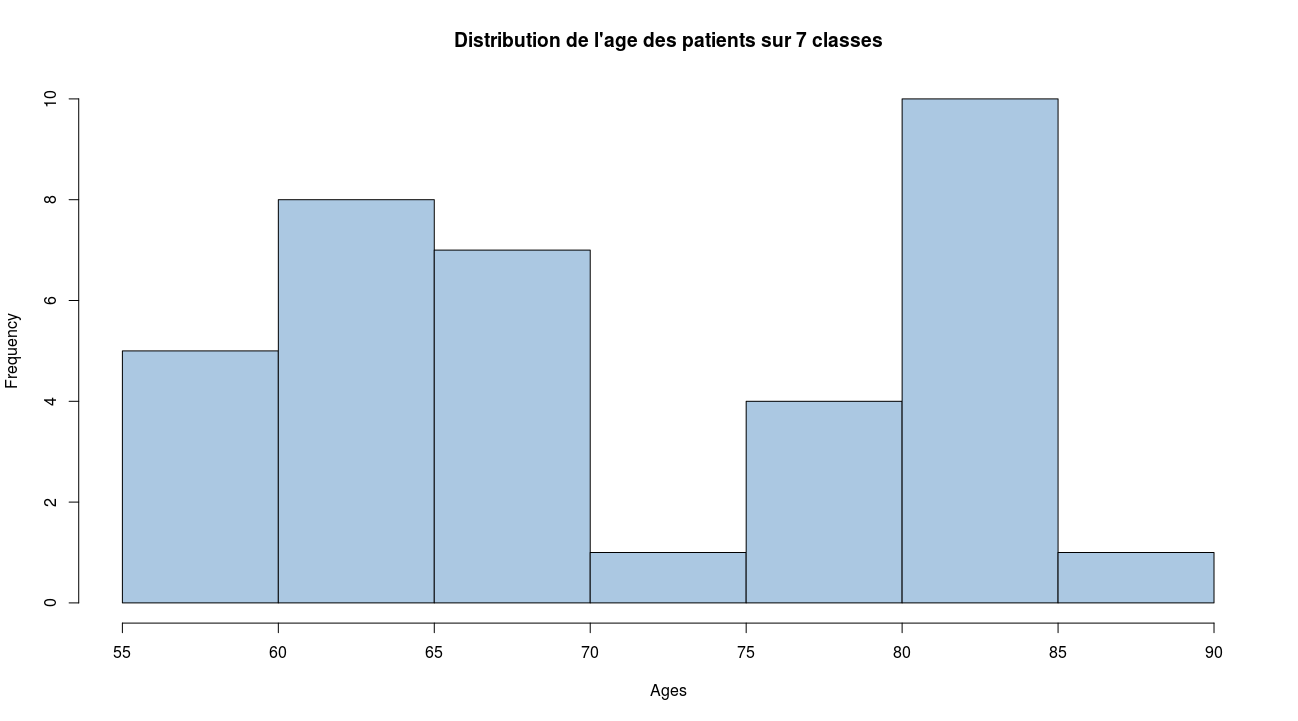
\includegraphics[width=1\textwidth]{../Fig/RTUPB/rtupb-age-frequency}
        \caption{RTUPB}
    \end{minipage}
    \hfill%
    \begin{minipage}[c]{.46\linewidth}
        \centering
        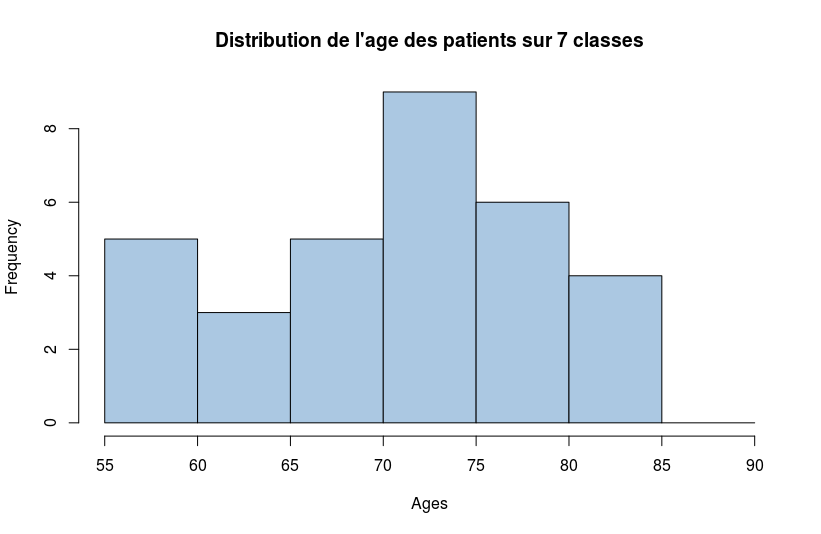
\includegraphics[width=1\textwidth]{../Fig/VPPBS/vppbs-age-frequency.png}
        \caption{VPPBS}
    \end{minipage}
\end{figure}


\begin{figure}[H]
\centering
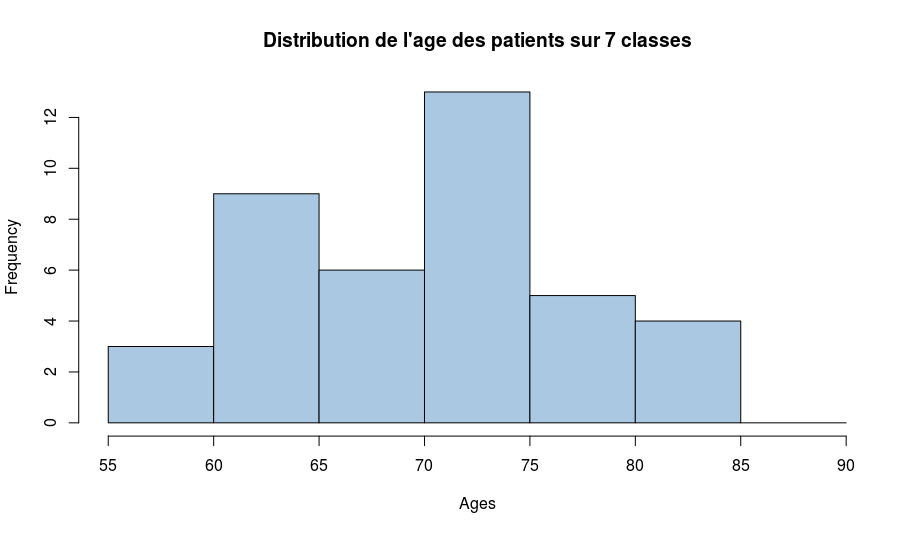
\includegraphics[width=0.50\textwidth]{../Fig/VAPOR/vapor-age-frequency}
\caption{VAPOR}
\end{figure}


%
%##########################
%# CONCLUSION
%##########################

%corrélations 
\subsection{Corrélation variables pré-opératoires}
  %"###############################################
%
% Corrélations 
%
%###############################################

Ici nous souhaitons mettre en évidence les corrélations possibles.
Nous limitons l’étude sur les tableaux post-opératoires des techniques RTUBD VPPBS et VAPOR contenant 
aussi les variables IPSS Qol et Qmax.
De même, certaines dimentions sont invariantes pour une technique donnée, nous avons supprimé celles-ci lors de la création 
de la matrice de corrélation et son corralélograme associé.

\begin{figure}[H]
\centering
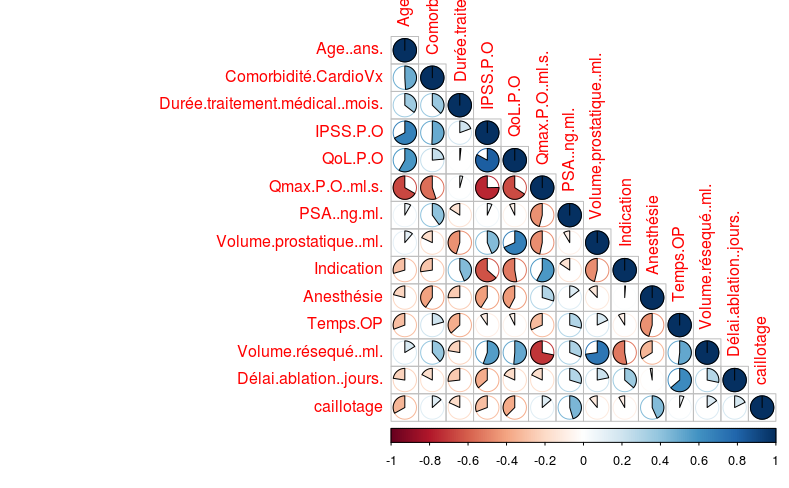
\includegraphics[width=0.75\textwidth]{../Fig/RTUPB/rtupb-corr-matrice-pie}
\caption{Matrice corrélation RTUBP}
\end{figure}

\begin{figure}[H]
\centering
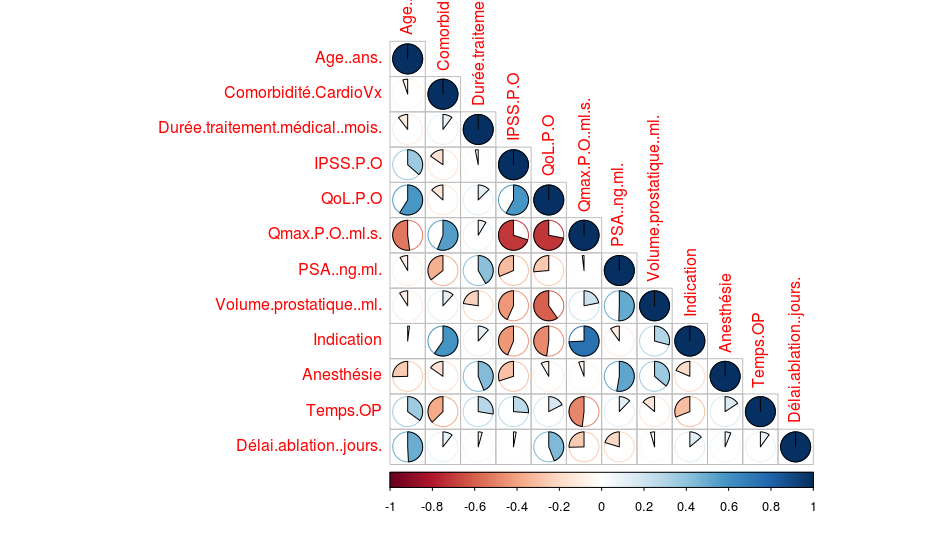
\includegraphics[width=0.75\textwidth]{../Fig/VPPBS/vppbs-corr-matrice-pie}
\caption{Matrice corrélation VPPBS}
\end{figure}

\begin{figure}[H]
\centering
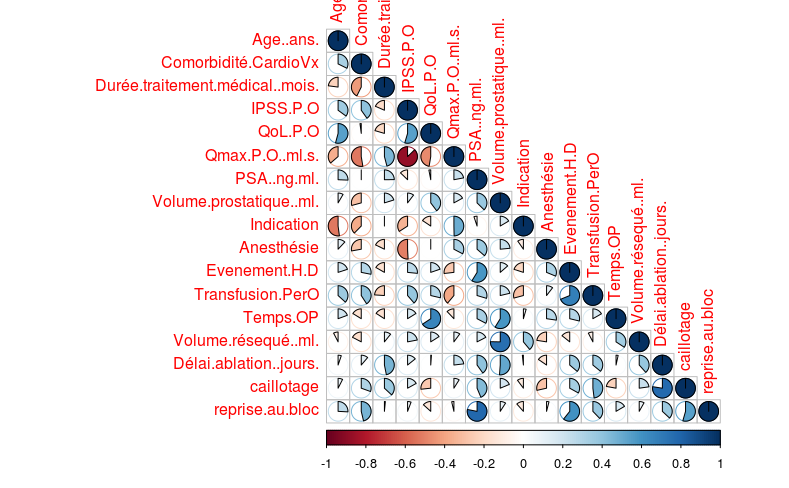
\includegraphics[width=0.75\textwidth]{../Fig/VAPOR/vapor-corr-matrice-pie}
\caption{Matrice corrélation VAPOR}
\end{figure}


Les variables  \emph{IPSS P.O} et   \emph{QoL P.O}  semblent avoir une corrélation qui peut sembler logique à la connaissance du fait qu’elles représentent pour l’une un indicateur de gène et pour l’autre un indicateur une qualité de vie post opératoire, même si c’est nettement plus marqué dans le cas de le panel des patients RTUBP. De même  pour les variables \emph{Volume prostatique} et \emph{Volume réséqué}. Aussi nous avons une corrélation \textbf{negative} intéressante entre le \emph{IPSS P.O} et le \emph{QMAX PO (ml/s)} (plus le patient à un QMax élevé moins il semble gêné alors que IPSS croît avec la gêne). 




%\begin{figure}[h]
%    \begin{minipage}[c]{.46\linewidth}
%        \centering
%        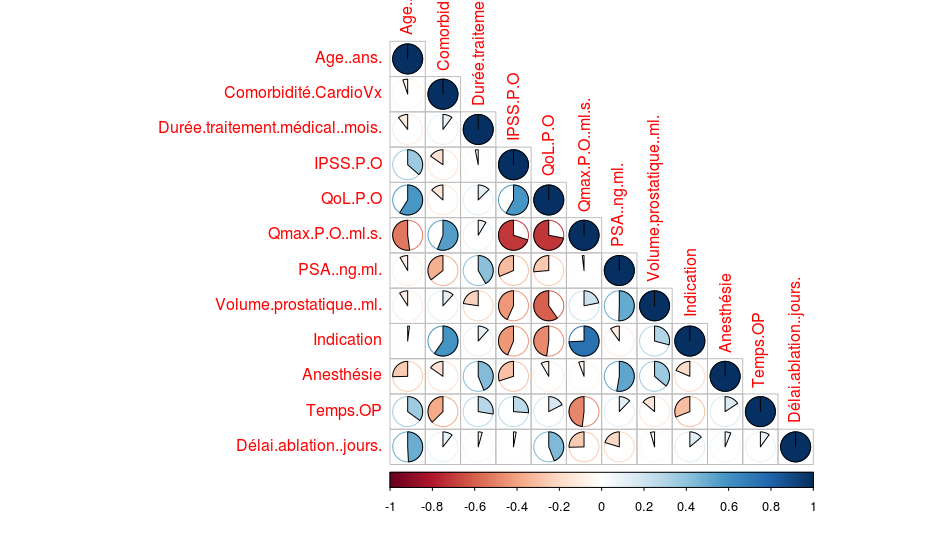
\includegraphics[width=1\textwidth]{../Fig/VPPBS/vppbs-corr-matrice-pie}
%        \caption{Légende}
%    \end{minipage}
%    \hfill%
%    \begin{minipage}[c]{.46\linewidth}
%        \centering
%        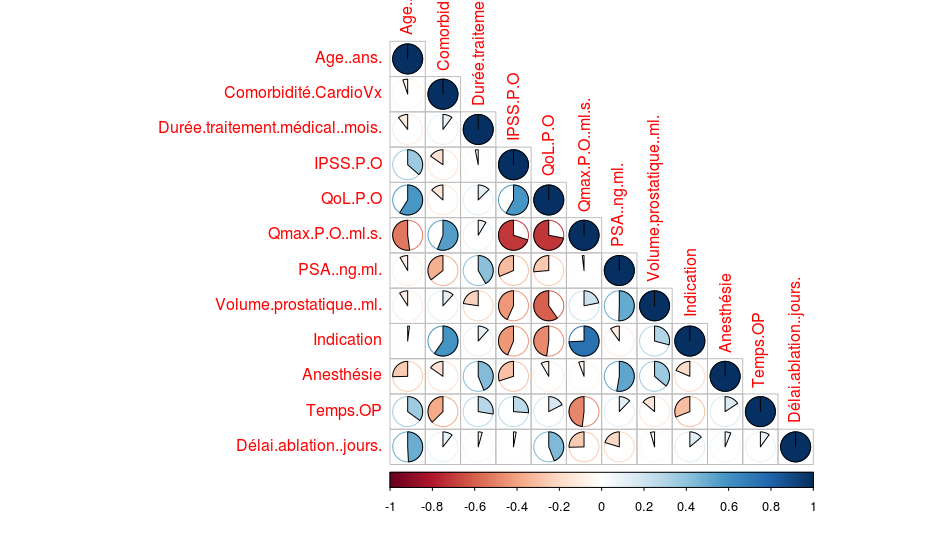
\includegraphics[width=1\textwidth]{../Fig/VPPBS/vppbs-corr-matrice-pie}
%        \caption{Légende}
%    \end{minipage}
%\end{figure}





%
%##########################
%# CONCLUSION
%##########################

\subsection{Distribution/évolution des données post-opératoires}
  %"###############################################
%
% IPSS
%
%###############################################

Dans l’analyse suivante nous souhaitons observer la distribution des variables IPSS Qol Et Qmax sur les différentes itérations temporelles fournies. L’objectif est de voir (pour l’ensemble des patients utilisant l’une des trois techniques ) comment cette distribution évolue.) 

\subsubsection{IPSS sur 18 mois }

RTUPB est une table composée de 36 patients. 
	
\begin{figure}[H]
\centering
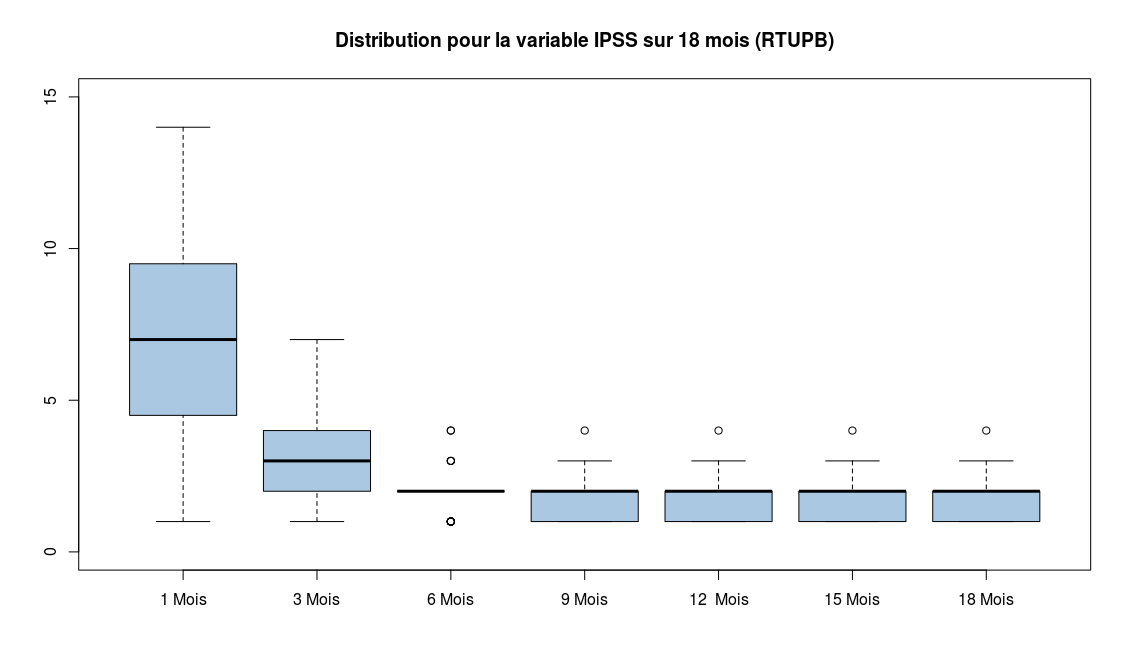
\includegraphics[width=0.75\textwidth]{../Fig/RTUPB/rtupb-boxplot-post-ipss}
\caption{RTUPB / IPSS sur 18 mois}
\end{figure}	
	
\begin{figure}[H]
\centering
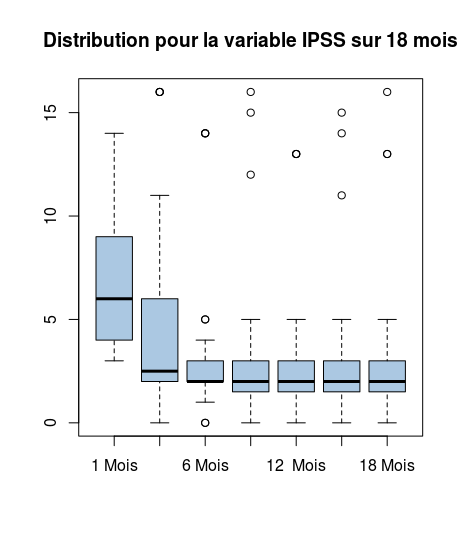
\includegraphics[width=0.75\textwidth]{../Fig/VPPBS/vppbs-boxplot-post-ipss}
\caption{VPPBS/IPSS sur 18 mois}
\end{figure}


\begin{figure}[H]
\centering
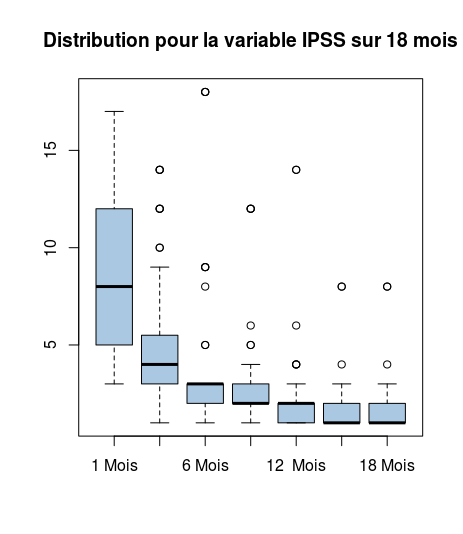
\includegraphics[width=0.75\textwidth]{../Fig/VAPOR/vapor-boxplot-post-ipss}
\caption{VAPOR/IPSS}
\end{figure}

%
%##########################
%# CONCLUSION
%##########################

Pour IPSS, l’on observe pour les trois techniques une décroissance de la valeur médiane dés le troisièmes mois. Dans le cadre de VAPOR et VPPBS, certains « outliers » sont présents (et ce sur l’ensemble des itérations dans le cadre de VPPBS ces « outliers » ont encore des valeurs très fortes même à partir du 18 mois.  RTUPB  semble avoir une variance homogène à partir du 9 ieme mois. Si VAPOR laisse apparaître des « ouliers », la valeur médiane termine plus bas que les deux autres techniques. 

  %"###############################################
%
% Qol 
%
%###############################################


\subsubsection{Qol sur 18 mois }

\begin{figure}[H]
\centering
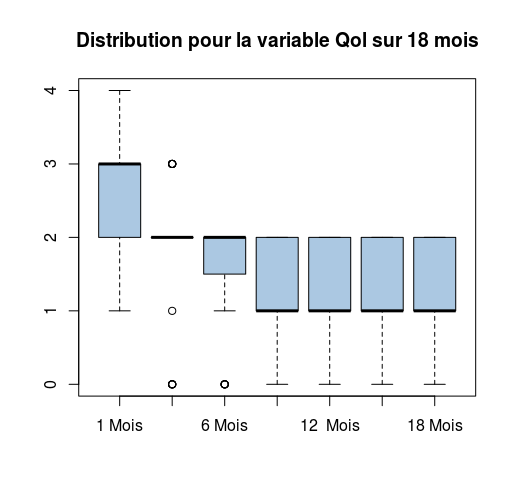
\includegraphics[width=0.75\textwidth]{../Fig/RTUPB/rtupb-boxplot-post-Qol}
\caption{RTUPB / Qol sur 18 mois}
\end{figure}	
	
\begin{figure}[H]
\centering
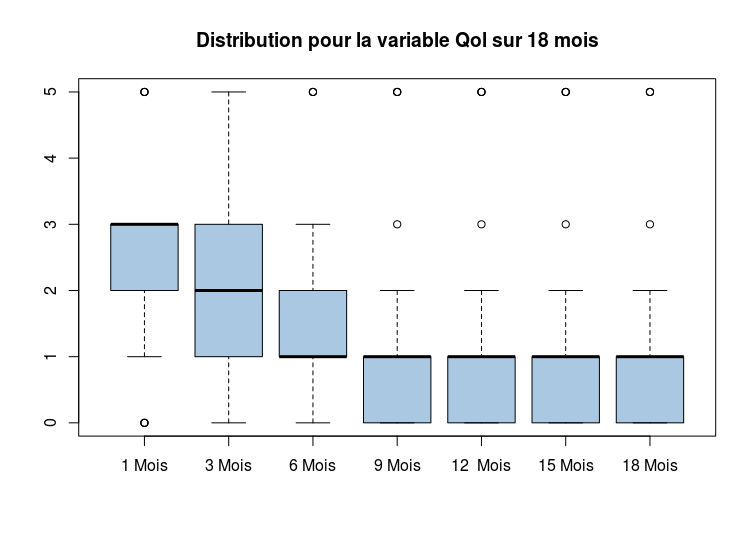
\includegraphics[width=0.75\textwidth]{../Fig/VPPBS/vppbs-boxplot-post-Qol}
\caption{VPPBS / Qol sur 18 mois}
\end{figure}	
	
	
\begin{figure}[H]
\centering
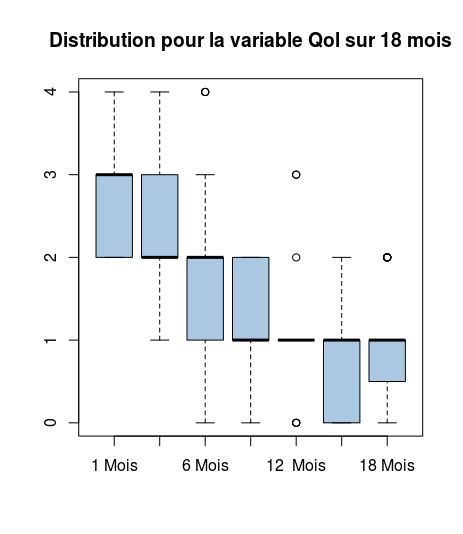
\includegraphics[width=0.75\textwidth]{../Fig/VAPOR/vapor-boxplot-post-Qol}
\caption{VAPOR / Qol sur 18 mois}
\end{figure}	
	


%
%##########################
%# CONCLUSION
%##########################
  %"###############################################
%
% Qmax
%
%###############################################

\subsubsection{Qmax sur 18 mois }

\begin{figure}[H]
\centering
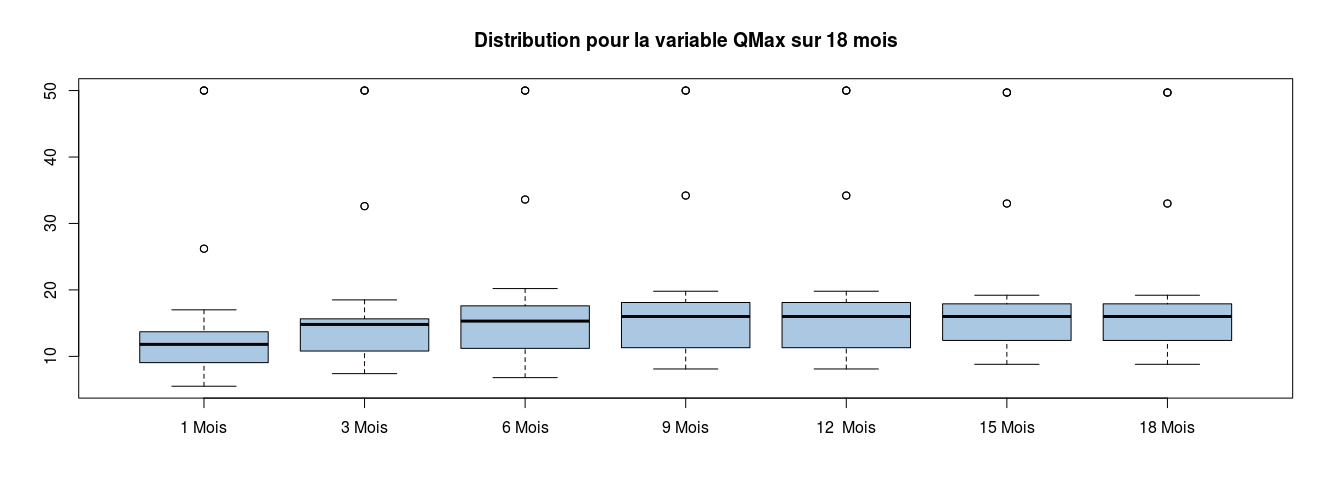
\includegraphics[width=0.75\textwidth]{../Fig/RTUPB/rtupb-boxplot-post-Qmax}
\caption{RTUPB / Qmax sur 18 mois}
\end{figure}	
	
\begin{figure}[H]
\centering
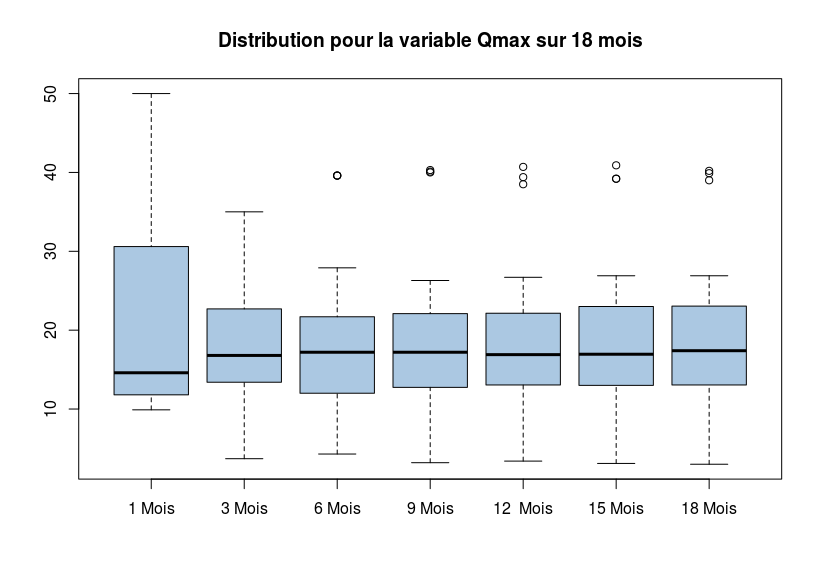
\includegraphics[width=0.75\textwidth]{../Fig/VPPBS/vppbs-boxplot-post-Qmax}
\caption{VPPBS/Qmax sur 18 mois}
\end{figure}


\begin{figure}[H]
\centering
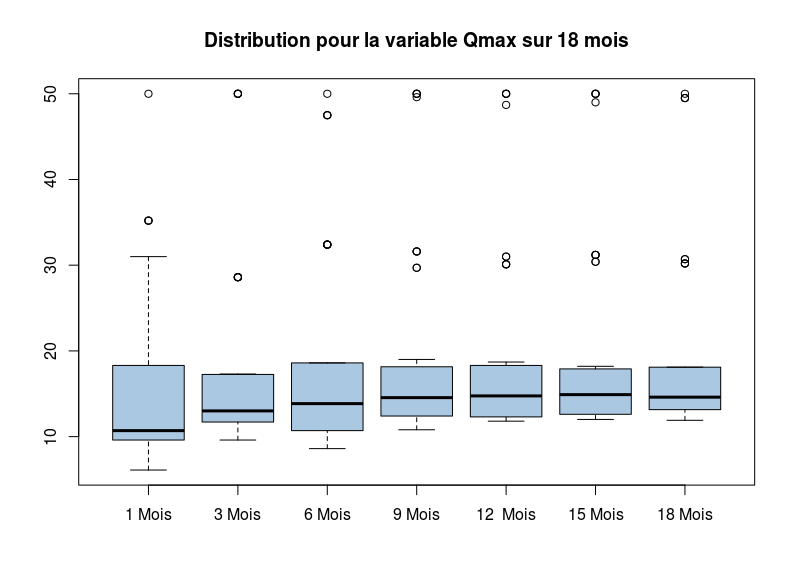
\includegraphics[width=0.75\textwidth]{../Fig/VAPOR/vapor-boxplot-post-Qmax}
\caption{VAPOR/Qmax}
\end{figure}

%
%##########################
%# CONCLUSION
%##########################

RTUPB semble être le plus constant, VPPBS permet d’obtenir de meilleurs résultats sur le Qmax (augmentation) avec des cas extrêmes plus élevés. VAPOR obtient des résultats médians proches de RTUPB mais avec des cas extrêmes plus élevés comparativement aux trois techniques.   
\newpage



%###############################################################
%Classification profils pre operatoires 
%###############################################################

\section{Classification profils pré-opératoires}

Dans le cadre de la classification nous avons observé quelques doublons, nous avons choisi de les supprimer 
du moins dans cette première phase. 


%vue d'ensemble 
\subsection{CAH / PAM RTUPB pré-opératoires }
	  %"###############################################
%
% Classification RTUPB pre 
%
%###############################################

\begin{figure}[H]
\centering
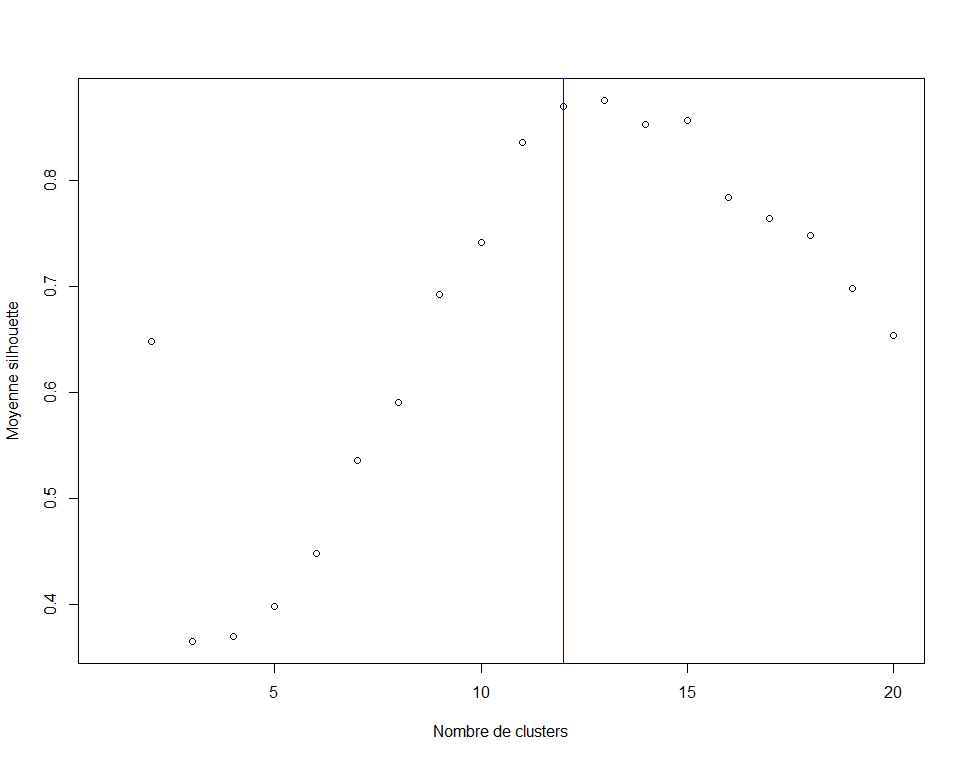
\includegraphics[width=0.90\textwidth]{../Fig/RTUPB/rtupb-elbow-pre.png}
\caption{RTUPB Maximise nb cluster / bonne classification}
\end{figure}

\begin{figure}[H]
\centering
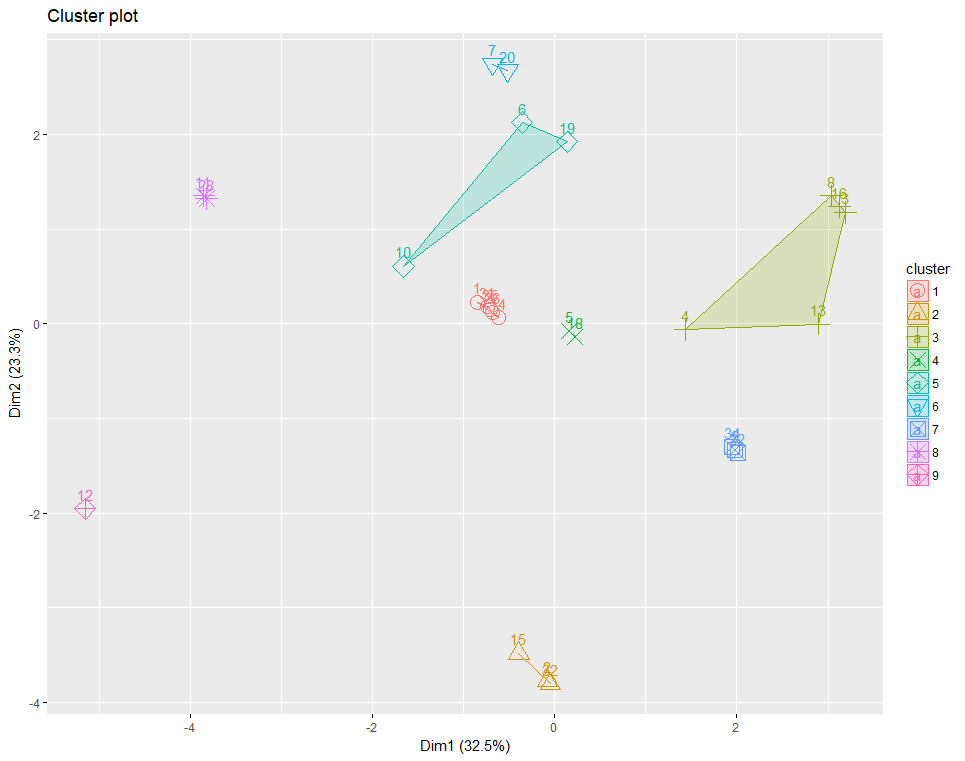
\includegraphics[width=0.90\textwidth]{../Fig/RTUPB/rtupb-pam-k12.png}
\caption{RTUPB Nuage de points / clusters PAM k=12 }
\end{figure}

\begin{figure}[H]
\centering
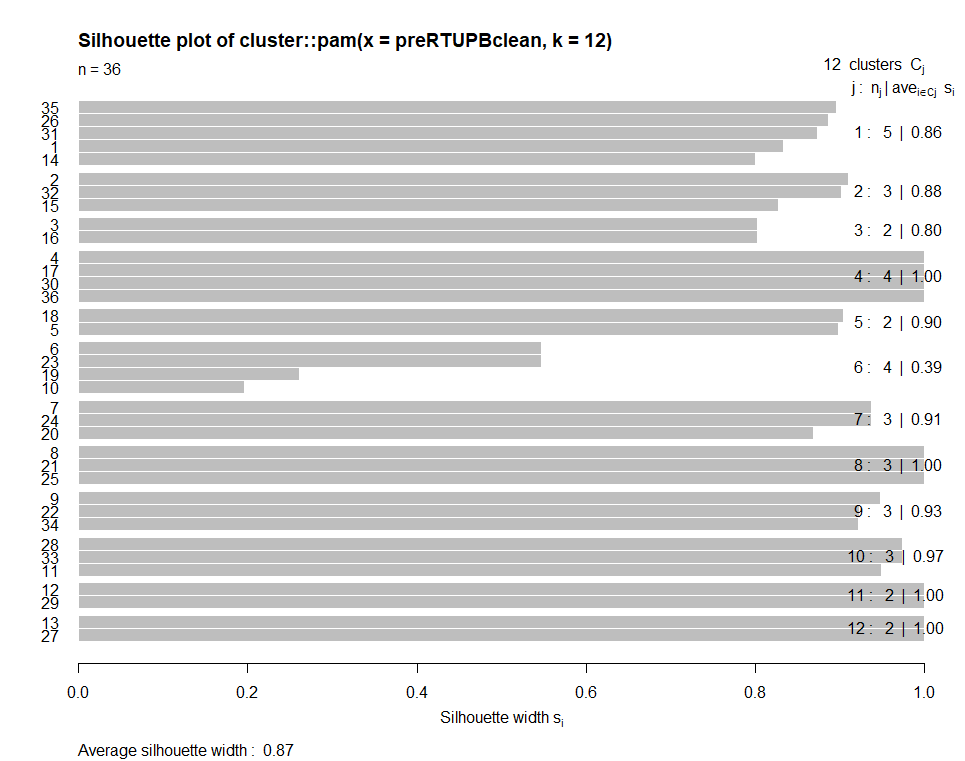
\includegraphics[width=0.90\textwidth]{../Fig/RTUPB/rtupb-sil-k12-pre.png}
\caption{RTUPB silhouette / clusters PAM k=12 }
\end{figure}

\begin{figure}[H]
\centering
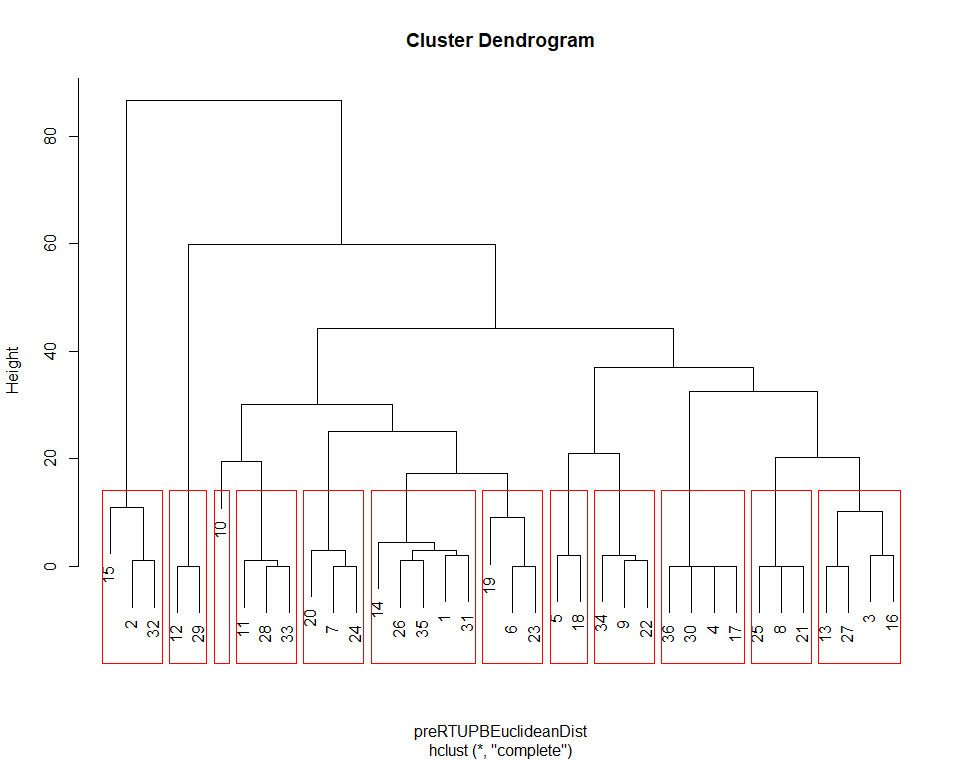
\includegraphics[width=0.90\textwidth]{../Fig/RTUPB/rtupb-cah-k12-pre.png}
\caption{RTUPB CAH séparation en k=12 }
\end{figure}


%"###############################################
%
% Interpretation des trois figures RTUPB pre 
%
%#############################################

Lors de notre analyse nous avons observé qu'il existait un ensemble d'individus similaires (ensemble des valeurs
identiques au relevé prés) ce qui s'observe dans la construction de certains clusters avec une valeur de qualité 
intra-cluster très forte en forgeant de petits clusters. Nous reviendrons sur ce point dans le rapprochement de ces
profils avec les profils de guérison ultérieurement. Nous avons estimé à 12 le nombre de clusters suivant la variation 
de la qualité globale  du cluster réalisé à partir de PAM. 

\textbf{Patients medoids 35, 2 ,16 ,36, 18, 23 ,24 ,25, 9, 33, 29 , 27}


%\begin{figure}[h]
%    \begin{minipage}[c]{.46\linewidth}
%        \centering
%        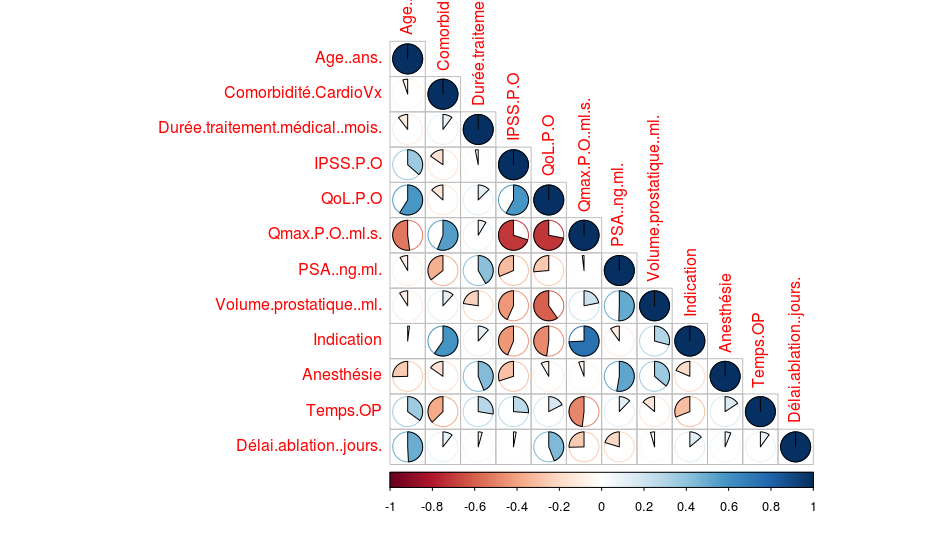
\includegraphics[width=1\textwidth]{../Fig/VPPBS/vppbs-corr-matrice-pie}
%        \caption{Légende}
%    \end{minipage}
%    \hfill%
%    \begin{minipage}[c]{.46\linewidth}
%        \centering
%        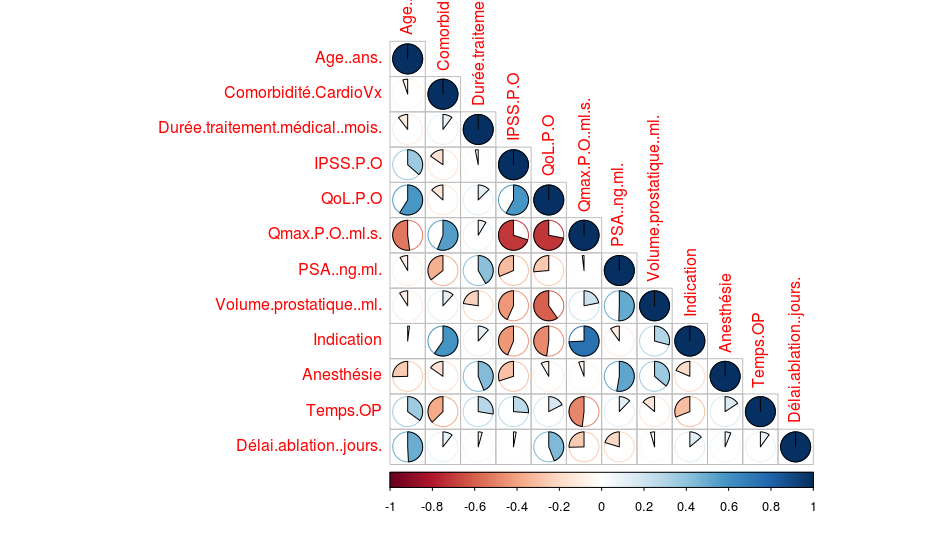
\includegraphics[width=1\textwidth]{../Fig/VPPBS/vppbs-corr-matrice-pie}
%        \caption{Légende}
%    \end{minipage}
%\end{figure}





%
%##########################
%# CONCLUSION
%##########################
  
\subsection{CAH / PAM VPPBS  pré-opératoires }
	  %"###############################################
%
% Classification VPBBS pre 
%
%###############################################

\begin{figure}[H]
\centering
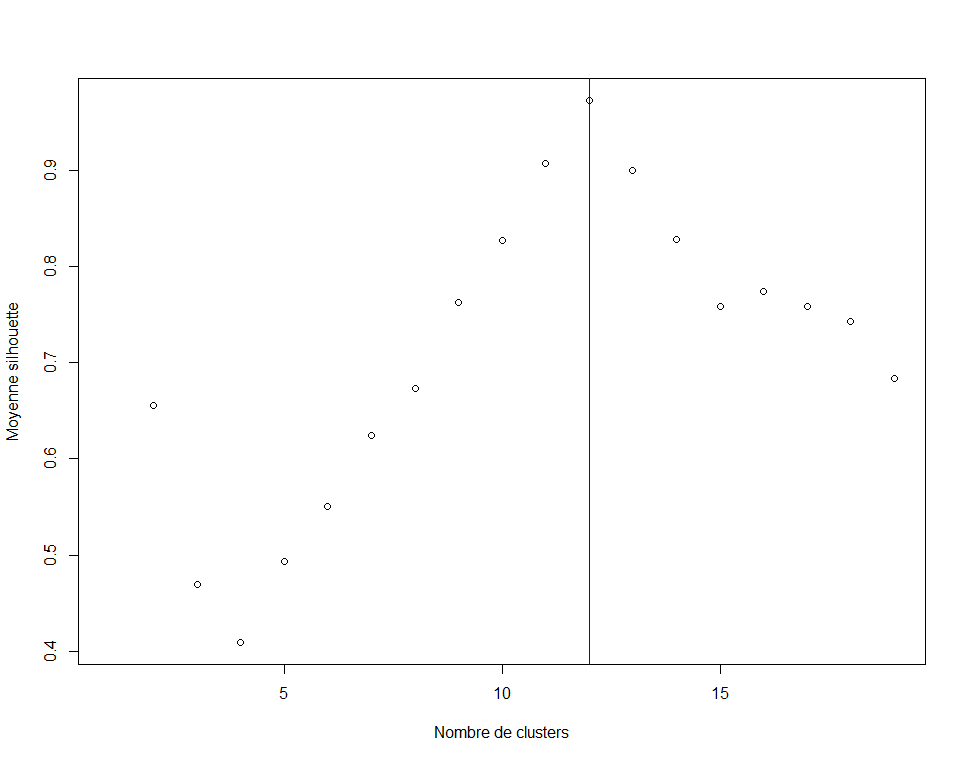
\includegraphics[width=0.90\textwidth]{../Fig/VPPBS/vppbs-elbow-pre.png}
\caption{VPPBS Maximise nb cluster / bonne classification}
\end{figure}

\begin{figure}[H]
\centering
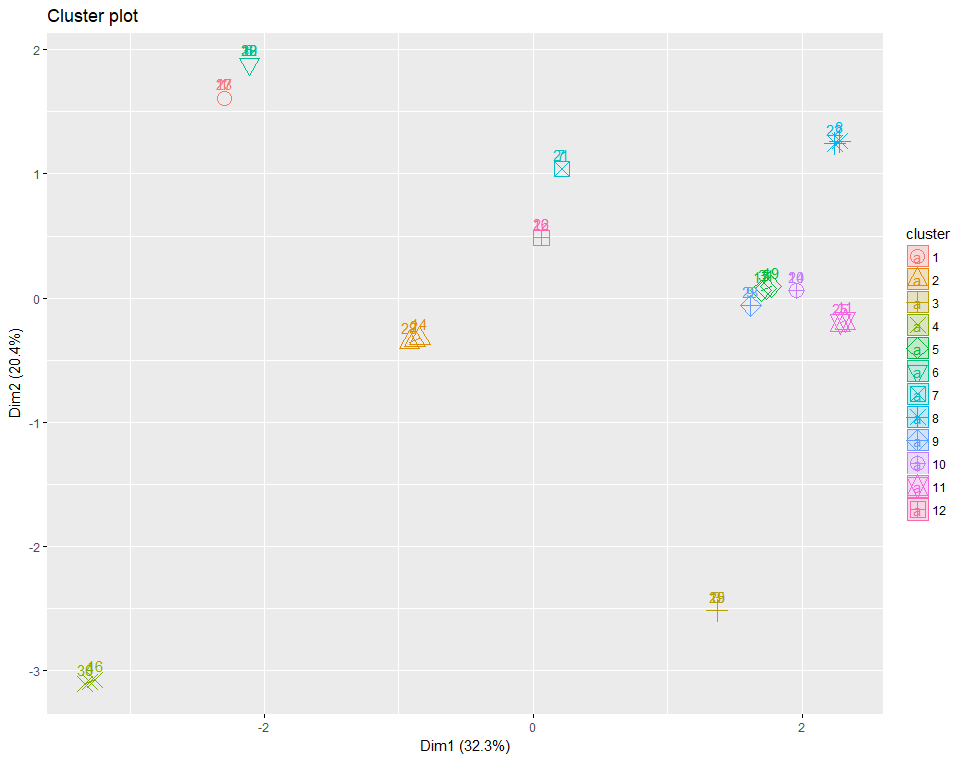
\includegraphics[width=0.90\textwidth]{../Fig/VPPBS/vppbs-pam-k12.png}
\caption{VPPBS Nuage de points / clusters PAM k=12 }
\end{figure}

\begin{figure}[H]
\centering
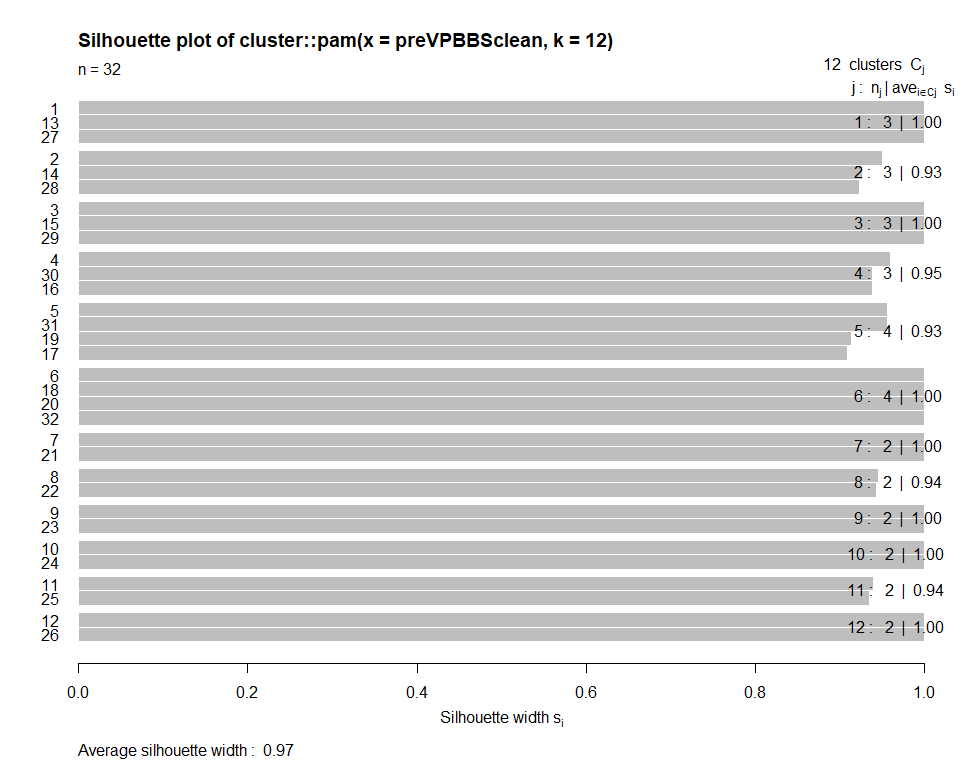
\includegraphics[width=0.90\textwidth]{../Fig/VPPBS/vppbs-sil-k12-pre.png}
\caption{VPPBS silhouette/ clusters PAM k=12 }
\end{figure}

%\begin{figure}[H]
\begin{figure}[H]
\centering
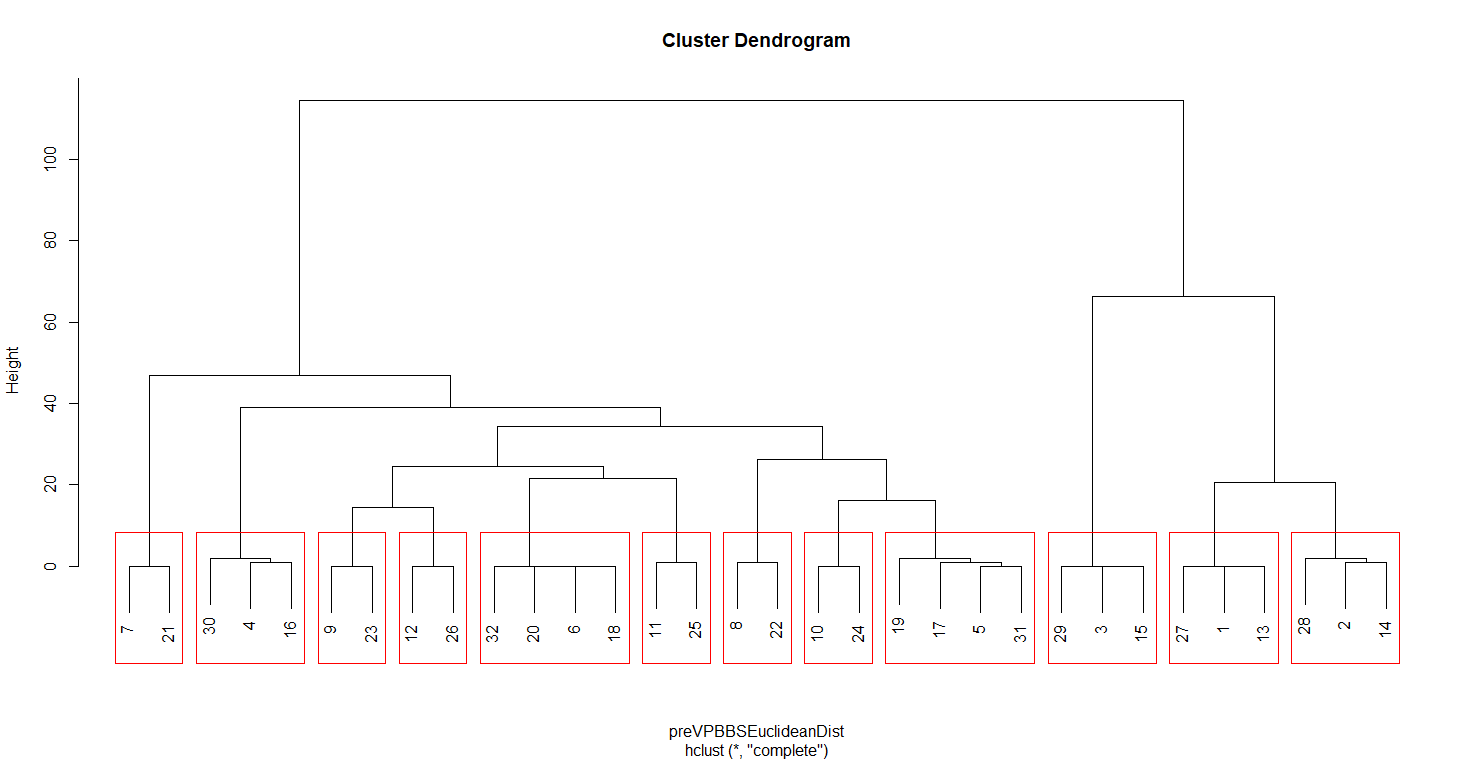
\includegraphics[width=0.90\textwidth]{../Fig/VPPBS/vppbs-cah-k12-pre.png}
\caption{VPPBS CAH séparation en k=12 }
\end{figure}


%"###############################################
%
% Interpretation des trois figures VPPBS pre 
%
%#############################################






%\begin{figure}[h]
%    \begin{minipage}[c]{.46\linewidth}
%        \centering
%        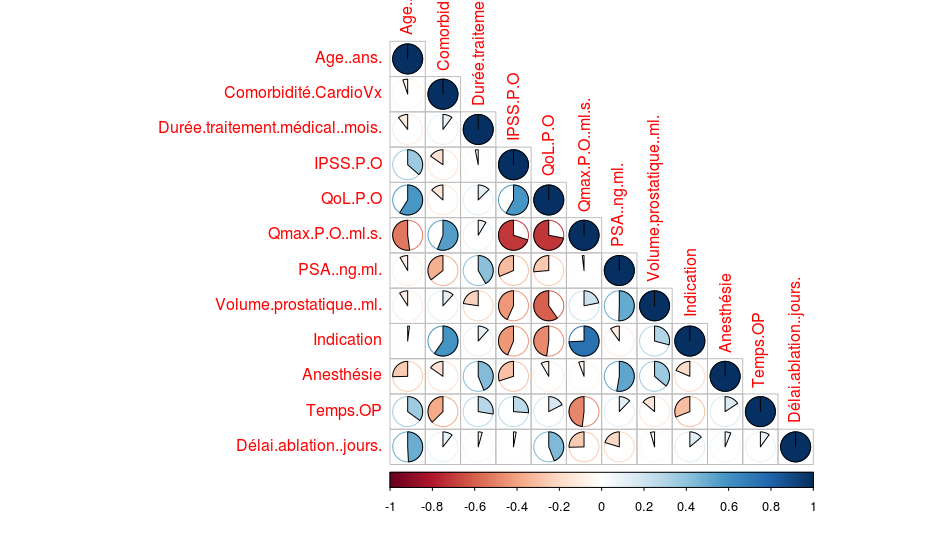
\includegraphics[width=1\textwidth]{../Fig/VPPBS/vppbs-corr-matrice-pie}
%        \caption{Légende}
%    \end{minipage}
%    \hfill%
%    \begin{minipage}[c]{.46\linewidth}
%        \centering
%        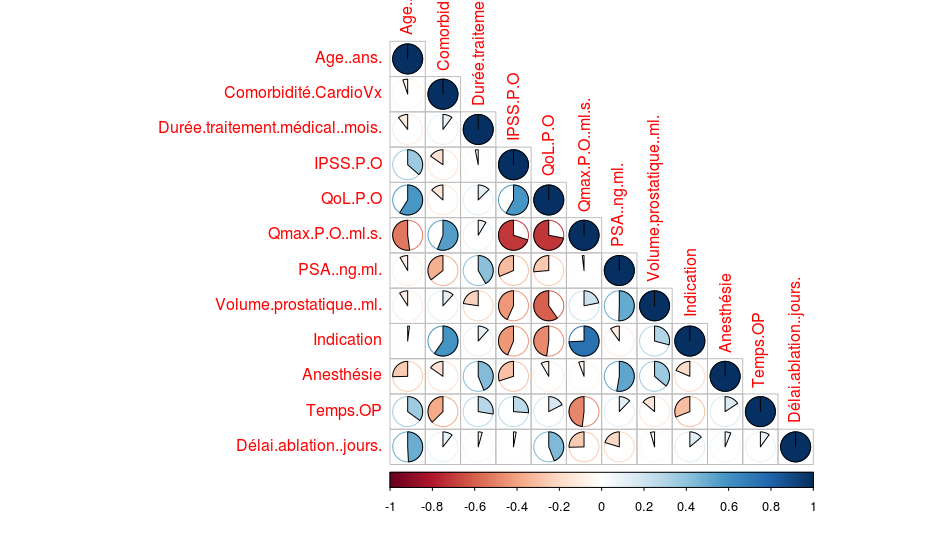
\includegraphics[width=1\textwidth]{../Fig/VPPBS/vppbs-corr-matrice-pie}
%        \caption{Légende}
%    \end{minipage}
%\end{figure}





%
%##########################
%# CONCLUSION
%##########################

\subsection{Comparaison Qmax }
	  %"###############################################
%
% Classification comparaison Qmax
%
%###############################################

\begin{figure}[h]
    \begin{minipage}[c]{.46\linewidth}
        \centering
        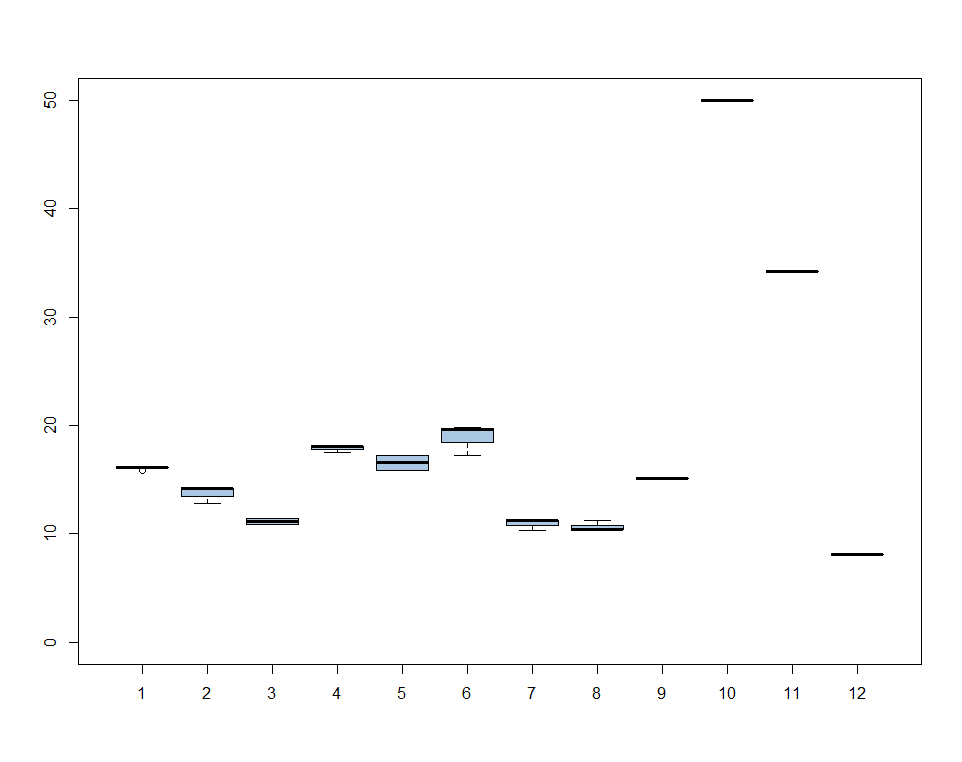
\includegraphics[width=1\textwidth]{../Fig/RTUPB/rtupb-qmax-k12-distribution.png}
        \caption{Distribution Qmax à 12 mois RTUPB}
    \end{minipage}
    \hfill%
    \begin{minipage}[c]{.46\linewidth}
        \centering
        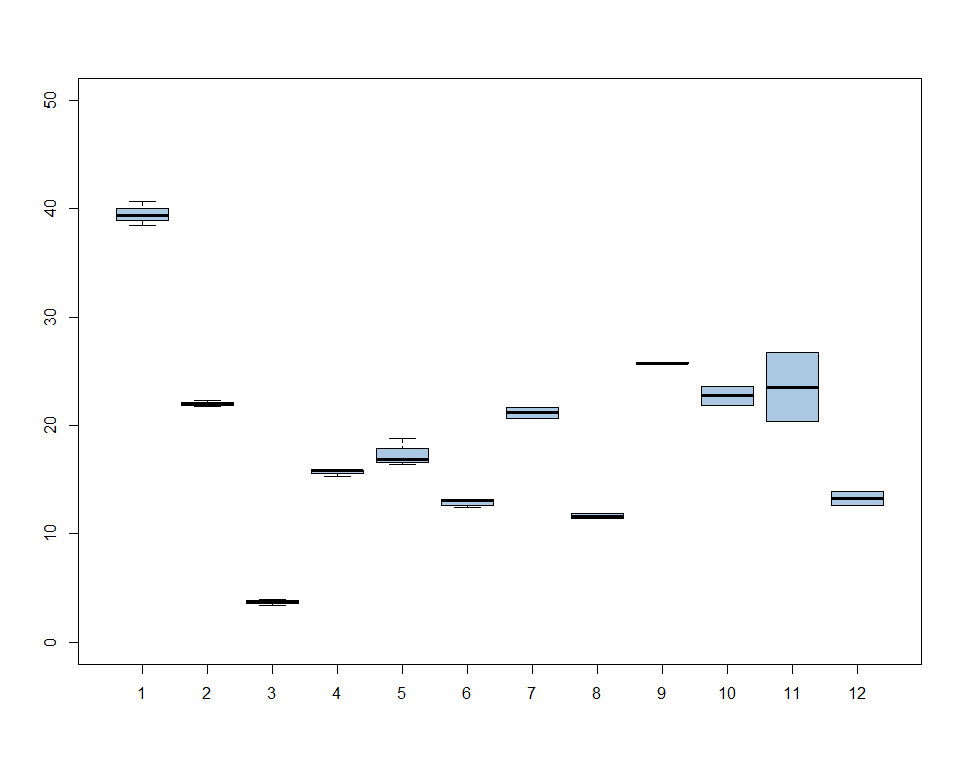
\includegraphics[width=1\textwidth]{../Fig/VPPBS/vppbs-qmax-k12-distribution.png}
        \caption{Distribution Qmax à 12 mois VPPBS}
    \end{minipage}
\end{figure}

%"###############################################
%
% Interpretation des trois figures RTUPB pre 
%
%#############################################




%\begin{figure}[h]
%    \begin{minipage}[c]{.46\linewidth}
%        \centering
%        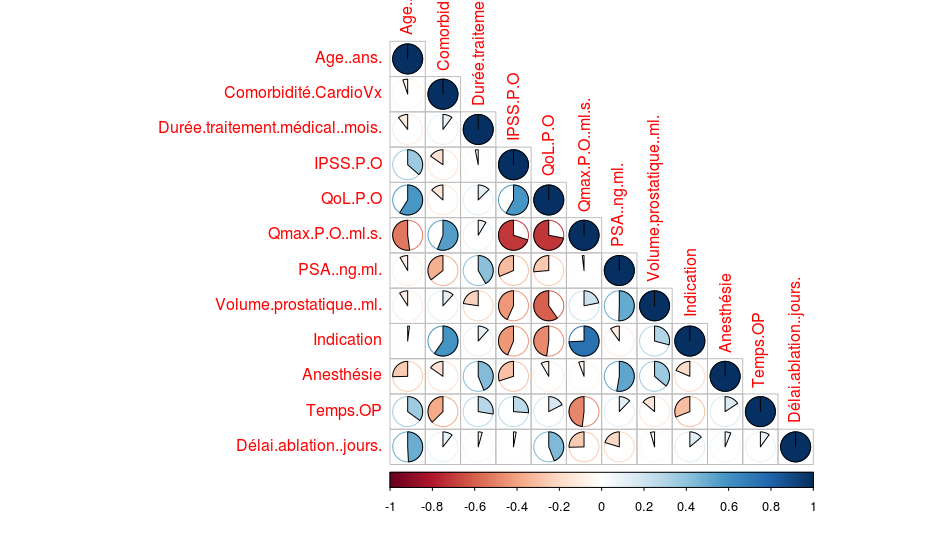
\includegraphics[width=1\textwidth]{../Fig/VPPBS/vppbs-corr-matrice-pie}
%        \caption{Légende}
%    \end{minipage}
%    \hfill%
%    \begin{minipage}[c]{.46\linewidth}
%        \centering
%        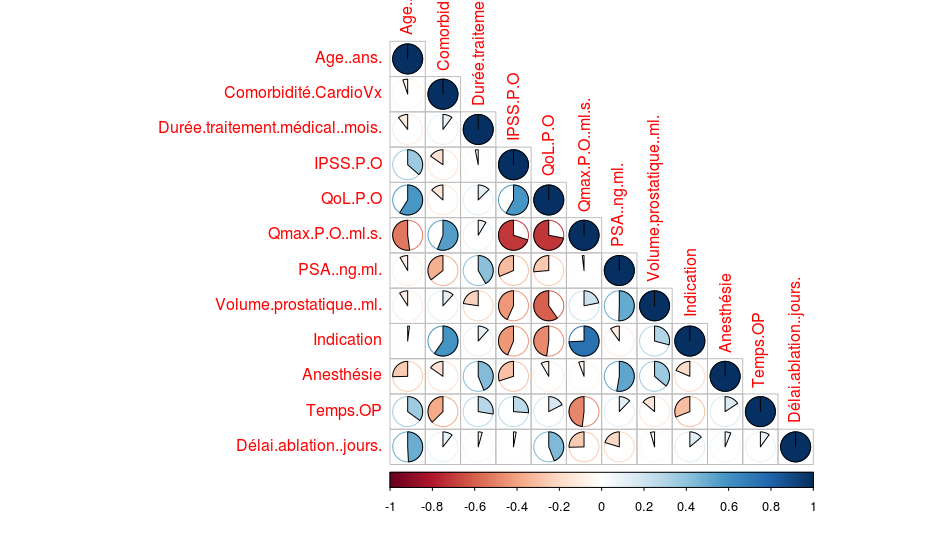
\includegraphics[width=1\textwidth]{../Fig/VPPBS/vppbs-corr-matrice-pie}
%        \caption{Légende}
%    \end{minipage}
%\end{figure}





%
%##########################
%# CONCLUSION
%##########################


%\section{Classification des profils pre op.}
%%###############################################
%# RTUPB
%###############################################
\subsection{Extraction des profils pour RTUPBS}

\subsubsection{QMax sur 12 mois}


%###############################################
%# RTUPBS
%###############################################
\subsection{Extraction des profils pour RTUPBS}

\subsubsection{QMax sur 12 mois}



%###############################################
%#QMAX 12 mois 
%###############################################
\subsection{Extraction des profils pour RTUPBS}

\subsubsection{Conclusion}
%\newpage


\section{Classification profils post-opératoires}
\subsection{CAH / PAM RTUPB post-opératoires}
	  %"###############################################
%
% Classification RTUPB post 
%
%###############################################

\begin{figure}[H]
\centering
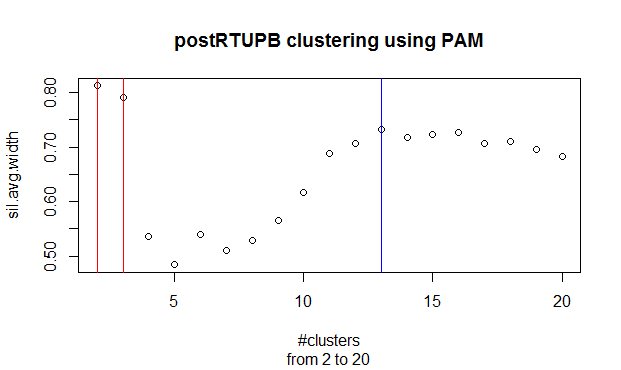
\includegraphics[width=0.90\textwidth]{../Fig/RTUPB/rtupb-elbow-post.png}
\caption{Maximisation de la silhouette moyenne }
\label{fig-rtupb-post-elbow}
\end{figure}

En utilisant PAM sur les données post-opératoires, la courbe des silhouettes moyennes
nous indique une valeur maximale pour un nombre de classes à k = 2 (Cf. figure~\ref{fig-rtupb-post-elbow}).

Cependant, si nous regardons le détail des classes et de leurs silhouettes pour k = 2 (Cf. figure~\ref{fig-rtupb-post-pam-k2}),
nous avons une première classe incluant la quasi totalité des patients dont 2 qui ont un profil post-opératoire non relié (valeurs de silhouette négatives), et une deuxième classe ne contenant que trois patients (11, 28 et 33)
avec une valeur de silhouette à 1, indiquant des données répliquées exactement et donc une classe triviale.
Après vérification que ces patients ont des données post-opératoires identiques, mais ne sont pas pour autant
des doublons (données pré-opératoires différentes), nous poursuivons la recherche jusqu'au maximum suivant qui se trouve à k = 3 (Cf. figure~\ref{fig-rtupb-post-elbow}).

\begin{figure}[H]
\centering
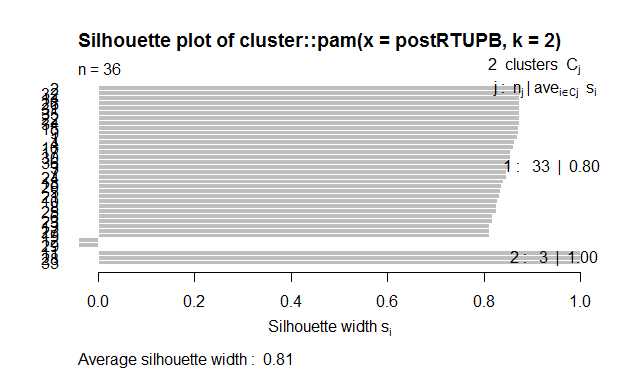
\includegraphics[width=0.75\textwidth]{../Fig/RTUPB/rtupb-sil-k2-post.png}
\caption{Silhouette / classe (k = 2) }
\label{fig-rtupb-post-pam-k2}
\end{figure}

En examinant, pour k = 3 (Cf. figure~\ref{fig-rtupb-post-pam-k3}), la répartition des classes et leurs silhouettes, nous faisons le même constat que précédemment, et une nouvelle classe triviale (patients 12 et 29) est apparue pour des patients distincts
mais dont les données post-opératoires sont identiques. Nous poursuivons encore la recherche jusqu'au maximum suivant qui se trouve à k = 13 (Cf. figure~\ref{fig-rtupb-post-elbow}).

\begin{figure}[H]
\centering
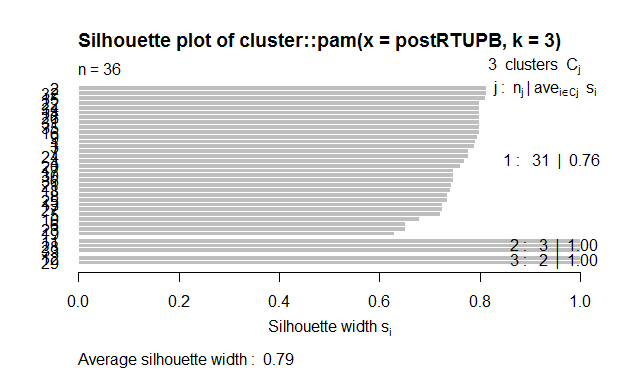
\includegraphics[width=0.75\textwidth]{../Fig/RTUPB/rtupb-sil-k3-post.png}
\caption{Silhouette / classe (k = 3)}
\label{fig-rtupb-post-pam-k3}
\end{figure}

Le partitionnement à 13 classes permet d'identifier 10 classes de profils post-opératoires bien voire très bien classés: 3 dont la silhouette vaut 1, 5 dont la silhouette est comprise entre 0.75 et 1, et 2 dont la silhouette
est aux alentours de 0.6). Ce partitionnement fait cependant apparaître 2 classes de profils post-opératoires pas très bien classés (silhouette < 0.5) et une classe singleton (silhouette = 0). 

\begin{figure}[H]
\centering
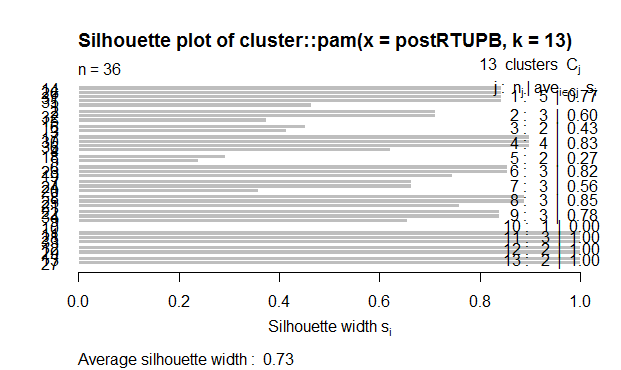
\includegraphics[width=0.75\textwidth]{../Fig/RTUPB/rtupb-sil-k13-post.png}
\caption{Silhouette / classe (k = 13)}
\label{fig-rtupb-post-pam-k13}
\end{figure}

La classification hiérarchique favoriserait plutôt un niveau de coupure de l'arbre correspondant à un partitionnement à 4 classes représenté en bleu sur la figure~\ref{fig-rtupb-post-cah}.
Un partitionnement avec des classes plus proches nous conduit à couper l'arbre au niveau suivant, ce qui
nous donne alors 13 classes. Ce partitionnement est représenté en bleu sur la figure~\ref{fig-rtupb-post-cah}.
Ce partitionnement à 13 classes correspond à celui obtenu par la méthode PAM, nous allons le retenir pour 
étudier dans la suite, les profils post-opératoires des patients médoïdes, et si cela se justifie après cela, nous refactoriserons en seulement 4 classes.

\begin{figure}[H]
\centering
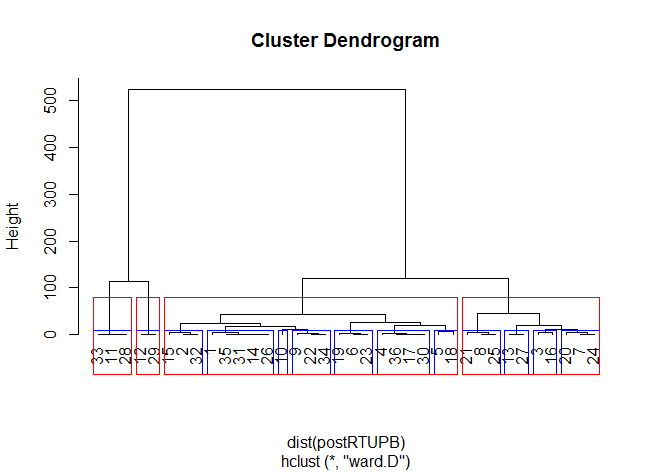
\includegraphics[width=0.75\textwidth]{../Fig/RTUPB/rtupb-cah-k13-post.png}
\caption{Silhouette / classe (k = 13)}
\label{fig-rtupb-post-cah}
\end{figure}


%
%##########################
%# CONCLUSION
%##########################
\subsection{CAH / PAM VPPBS post-opératoires}
	  %"###############################################
%
% Classification VPPBS post 
%
%###############################################

Pour rechercher le nombre optimal de classes, nous avons évalué, figure~\ref{fig-vppbs-post-elbow} la silhouette moyenne des classes pour un partitionnement de 2 à 20 classes. Il en ressort un pic net (en rouge) à 4 classes, mais la valeur maximale de la silhouette moyenne est atteinte pour k = 12 classes.

\begin{figure}[H]
\centering
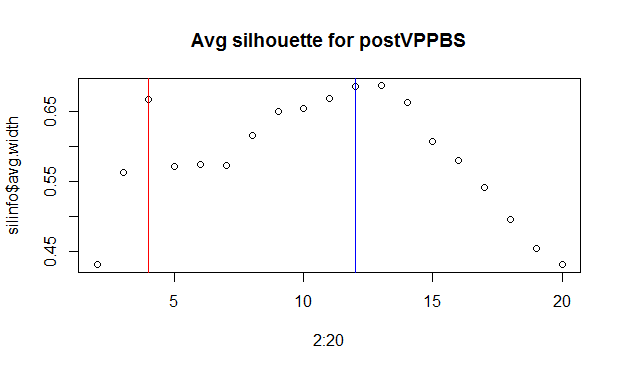
\includegraphics[width=0.75\textwidth]{../Fig/VPPBS/vppbs-elbow-post.png}
\caption{Recherche du meilleur nombre de classes}
\label{fig-vppbs-post-elbow}
\end{figure}

Jetons un bref coup d'oeil sur les silhouettes de classes pour le partitionnement à 4 classes (Cf. figure \ref{fig-vppbs-post-pam-k4}. Nous pouvons y observer 3 classes très solides (valeurs de silhouette entre 0.9 et 1), non triviales (contrairement à certaines classes observées pour les données post-opératoires RTUPB), et chacune de ces classes compte 3 ou quatre patients ; la quatrième classe rassemble tous les autres profils (22 patients sur 32), avec une silhouette de classe assez faible (0.55). Les 3 premières classes observées ici se détachent nettement et nous les retrouverons donc dans le partitionnement à k = 12 classes qui, compte tenu de la silhouette moyenne maximale, devrait faire apparaître de nouvelles classes parmi les 22 profiles restant. Les silhouettes correspondant à ce partitionnement à 12 classes font ressortir, figure~\ref{fig-vppbs-post-pam-k12}:
\begin{itemize}
\item 6 classes de profils fortement corrélés (silhouette > 0.7)
\item seulement 2 classes de profils peu ou pas corrélés (silhouette < 0.5)
\end{itemize}

\begin{figure}[H]
\centering
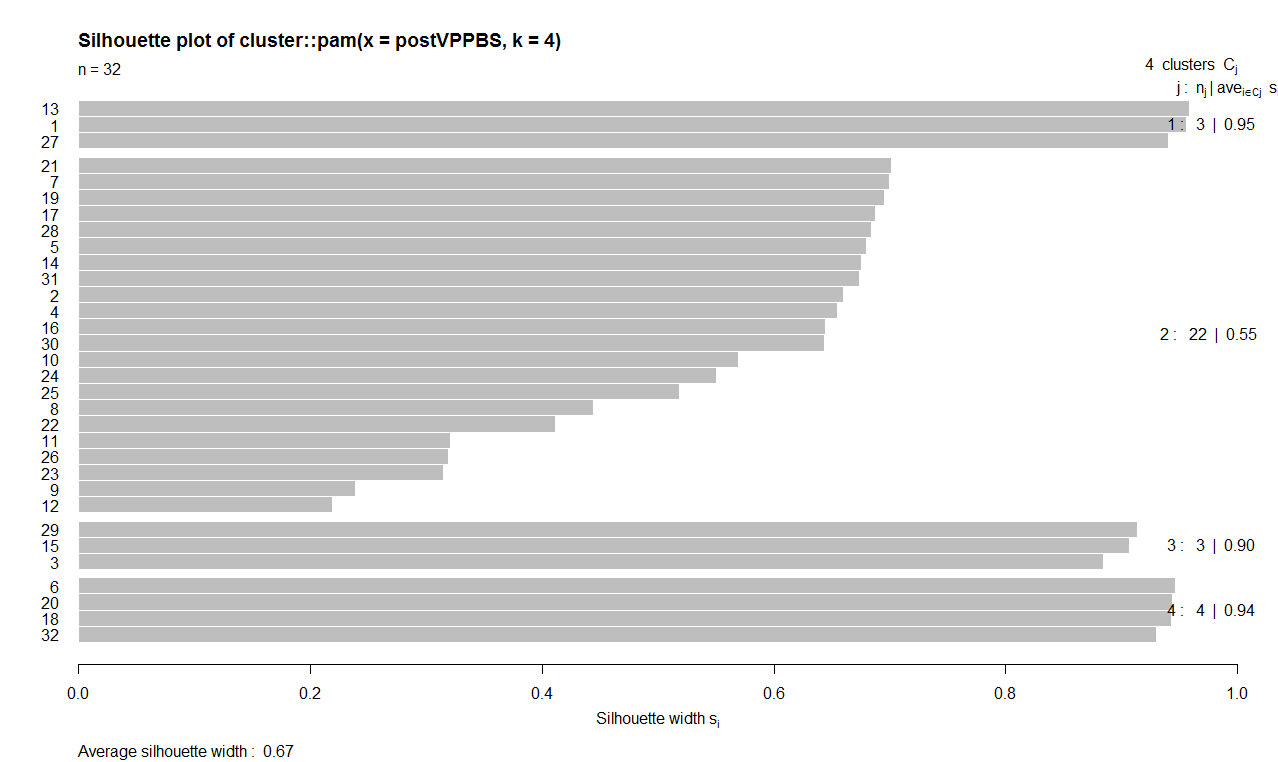
\includegraphics[width=0.75\textwidth]{../Fig/VPPBS/vppbs-sil-k4-post.png}
\caption[]{Silhouette / classe (k = 4)}
\label{fig-vppbs-post-pam-k4}
\end{figure}


\begin{figure}[H]
\centering
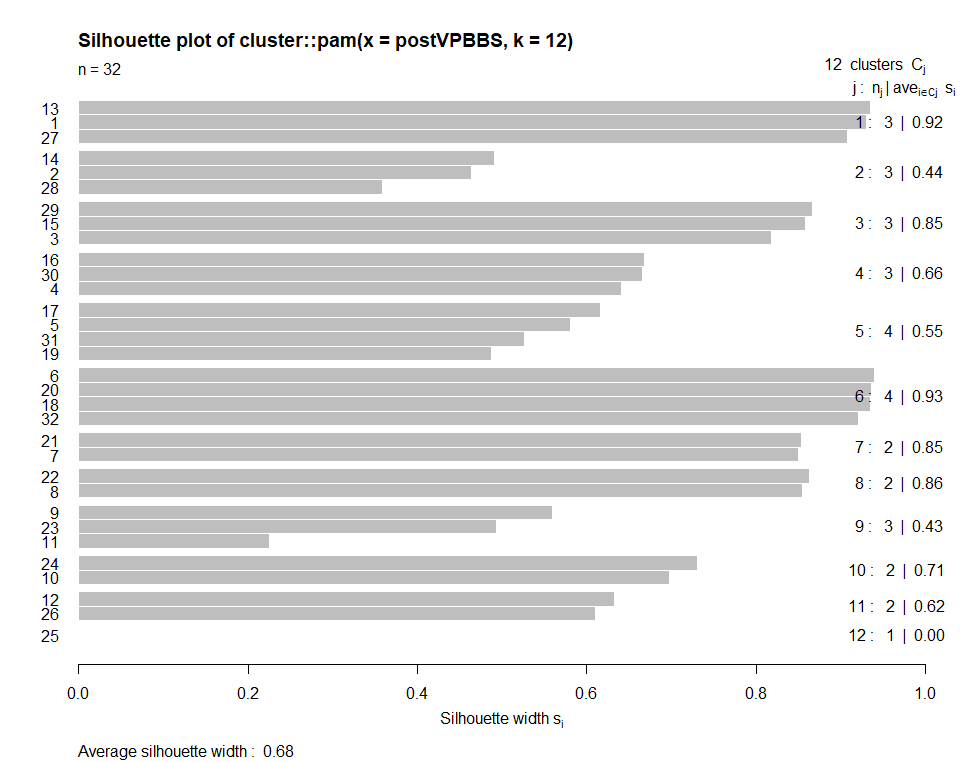
\includegraphics[width=0.75\textwidth]{../Fig/VPPBS/vppbs-sil-k12-post.png}
\caption{Silhouette / classe (k = 12)}
\label{fig-vppbs-post-pam-k12}
\end{figure}

La classification hiérarchique des données post-opératoires VPPBS produit le dendogramme présenté figure~\ref{fig-vppbs-post-cah}. La coupure de l'arbre peut s'effectuer soit à 5 classes (représentées en rouge), soit à 12 classes (représentées en bleu). Le partitionnement à 12 classes correspondant à celui obtenu par la méthode, nous le retiendrons pour étudier les profils post-opératoires. Au besoin, si cela se justifie par la suite, nous factoriserons pour revenir à un partitionnement à 5 classes.

\begin{figure}[H]
\centering
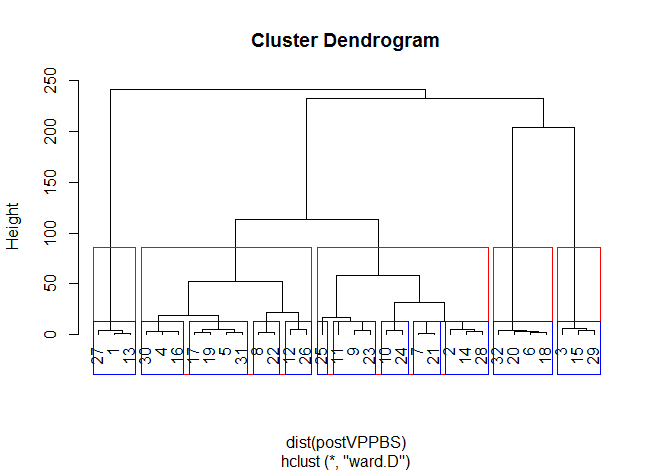
\includegraphics[width=0.75\textwidth]{../Fig/VPPBS/vppbs-cah-k12-post.png}
\caption{VPPBS: Classification hiérarchique}
\label{fig-vppbs-post-cah}
\end{figure}

%
%##########################
%# CONCLUSION
%##########################
\subsection{Profils pré-opératoires}
	  %###############################################
%# RTUPB
%###############################################
\subsection{Extraction des profils pour RTUPBS}

\subsubsection{QMax sur 12 mois}


%###############################################
%# RTUPBS
%###############################################
\subsection{Extraction des profils pour RTUPBS}

\subsubsection{QMax sur 12 mois}



%###############################################
%#QMAX 12 mois 
%###############################################
\subsection{Extraction des profils pour RTUPBS}

\subsubsection{Conclusion}
\subsection{Profils post-opératoires}
	  %"###############################################
%
% Profils post opératoires
%
%###############################################


TBD



%
%##########################
%# CONCLUSION
%##########################
\subsection{Liens entre profils pré et post-opératoires}
	  %
%##########################
%# LIENS INTER-PROFILS
%##########################

\subsubsection{Liens entre profils pré et post-opératoires}

Pour comparer les résultats précédents et les profils identifiés, nous reprenons et rapprochons pour chaque patient son profil pré-opératoire et son profil post-opératoire. La liste des couples de profils ainsi obtenue
est triée
\begin{itemize}
 \item  par profil pré-opératoire~: figure~\ref{fig-rtupb-histogram} et figure~\ref{fig-vppbs-histogram} pour respectivement RTUPB et VPPBS
 \item  par profil post-opératoire~: figure~\ref{fig-rtupb-histogram2} et figure~\ref{fig-vppbs-histogram2} pour respectivement RTUPB et VPPBS
\end{itemize}

\begin{figure}[H]
\centering
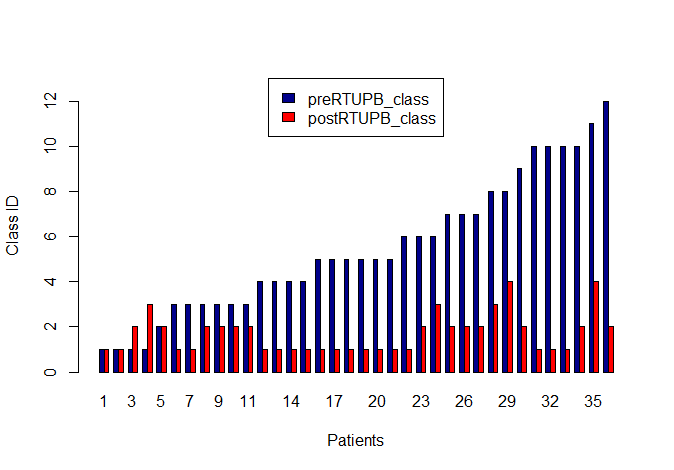
\includegraphics[width=0.75\textwidth]{../Fig/RTUPB/rtupb-histogram-pre-post.png}
\caption{RTUPB: classes post-opératoires en fonction des classes pré-opératoires}
\label{fig-rtupb-histogram}
\end{figure}

La figure~\ref{fig-rtupb-histogram} révèle que pour les patients appartenant au profil pré-opératoire 4, 5 et 7 le résultat constaté est toujours le profil post-opératoire n°1.  Pour les autres profils pré-opératoires (à l'exception des singletons pour lesquels les résultats ne sont donc pas confirmés), il n'existe pas de profils post-opératoires uniques permettant d'en déduire une prévision de guérison.
La figure~\ref{fig-rtupb-histogram2} n'apporte pas d'informations complémentaires.

\begin{figure}[H]
\centering
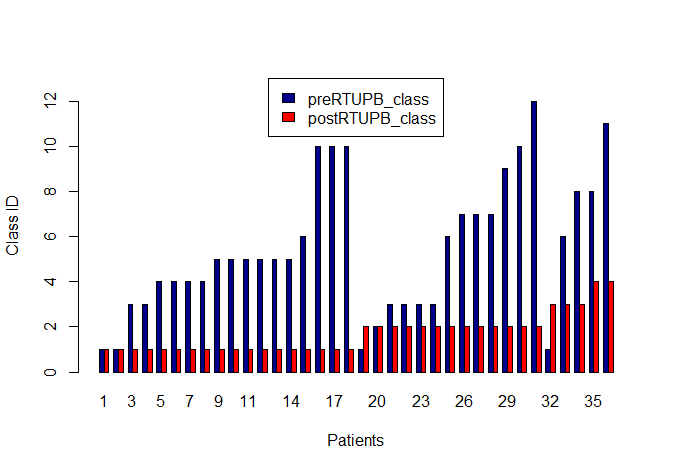
\includegraphics[width=0.75\textwidth]{../Fig/RTUPB/rtupb-histogram-post-pre.png}
\caption{RTUPB: classes pré-opératoires en fonction des classes post-opératoires}
\label{fig-rtupb-histogram2}
\end{figure}

Pour VPPBS, la figure~\ref{fig-vppbs-histogram} montre la correspondance d'un seul profil post-opératoire pour chaque profil pré-opératoire. Nous pouvons donc nous baser sur le profil pré-opératoire pour envisager ou non une opération VPPBS et prévoir la guérison.

\begin{figure}[H]
\centering
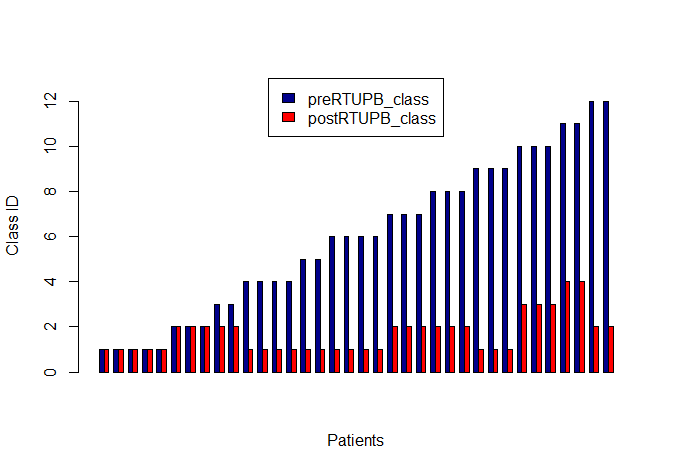
\includegraphics[width=0.75\textwidth]{../Fig/VPPBS/vppbs-histogram-pre-post.png}
\caption{VPPBS: classes post-opératoires en fonction des classes pré-opératoires}
\label{fig-vppbs-histogram}
\end{figure}

\begin{figure}[H]
\centering
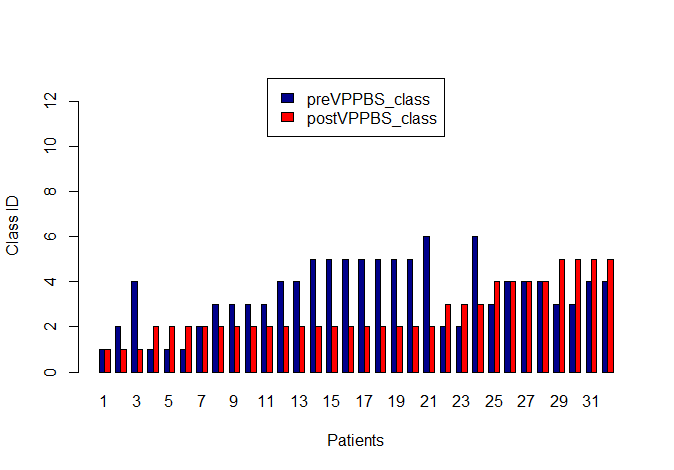
\includegraphics[width=0.75\textwidth]{../Fig/VPPBS/vppbs-histogram-post-pre.png}
\caption{VPPBS: classes pré-opératoires en fonction des classes post-opératoires}
\label{fig-vppbs-histogram2}
\end{figure}


\section{Classification supervisée RTUPB-VPPBS et VAPOR}
\subsection{RTUPB: prédiction IPSS, QoL et Qmax à 12 mois}
	  %"###############################################
%
% Classification supervisée
%
%###############################################

% RTUPB: variables post-op à 12 mois
%
%###############################################

Dans les sections qui suivent, nous réutilisons la même méthode pour construire un arbre de régression:
pour chacune des techniques opératoires (respectivement RTUPB, VPPBS et VAPOR) et à partir des données pré-opératoires précédemment utilisées et nettoyées des variables invariantes ou incomplètes, auxquelles on ajoutera la variable à prédire, nous effectuons un tirage aléatoire pour créer deux ensembles de données:
\begin{itemize}
\item un ensemble d'apprentissage représentant 80\% des patients opérés par une technique. A partir de cet ensemble, nous inférerons un arbre de régression en utilisant le package rpart sous R.
\item un ensemble de validation représentant 20\% des patients opérés par la même technique.
\end{itemize}
Les variables IPSS et QoL seront traitées comme des variables ordinales, tandis que la variable Qmax sera
traitée comme une variable linéaire.

Pour chaque variable et chaque base, nous comparerons les résultats obtenus par un arbre de régression (inféré par élagage d'un arbre "complet") et les résultats obtenus par une forêt aléatoire d'arbres de régression.

\subsubsection{RTUPB: IPSS à 12 mois}

L'arbre de régression complet obtenu pour la variable IPSS à 12 mois (colonne IPSS\_\_4) met en {\oe}uvre 6 variables (Cf. figure~\ref{fig-rtupb-full-regtree-ipss12}).
Les feuilles de l'arbre représentent, en première ligne, la valeur prédite (la plus probable) pour IPSS à 12 mois. La ligne suivante indique les probabilités pour chacun des 3 niveaux constatés sur l'échantillon d'apprentissage pour IPSS à 12 mois, c'est-à-dire respectivement 1/2/3. Par exemple en cas de caillotage (valeur == 1), l'arbre de régression conduit à la feuille en bas à gauche et prédit une valeur IPSS à 1 avec une probabilité de 88\%.

\begin{figure}[H]
\centering
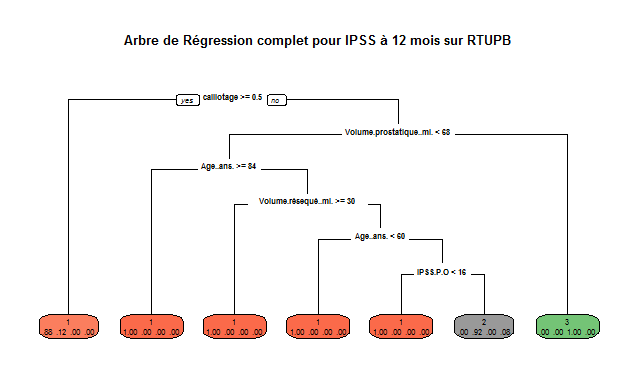
\includegraphics[width=0.75\textwidth]{../Fig/RTUPB/rtupb-full-regtree-ipss12.png}
\caption{RTUPB: Arbre de régression pour IPSS à 12 mois}
\label{fig-rtupb-full-regtree-ipss12}
\end{figure}

Afin de simplifier l'arbre, nous vérifions le facteur d'amélioration (complexity parameter) apporté par chaque embranchement de l'arbre, figure~\ref{fig-rtupb-regtree-optim-ipss12}. Nous élaguons l'arbre au niveau du coude d'inflexion de la courbe, soit environ à cp=0.13, pour obtenir un arbre simplifié  (figure~\ref{fig-rtupb-regtree-predict-ipss12}).

\begin{figure}[H]
\centering
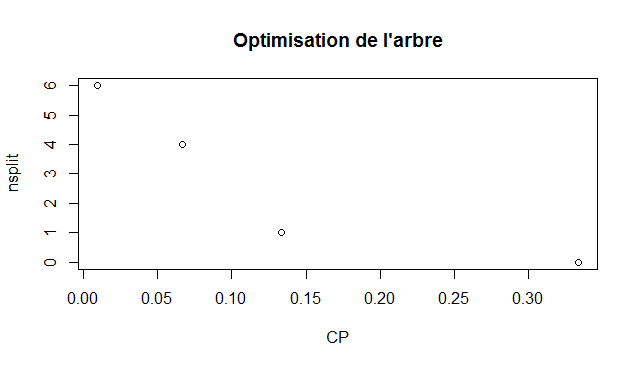
\includegraphics[width=0.75\textwidth]{../Fig/RTUPB/rtupb-regtree-optim-ipss12.png}
\caption{RTUPB: Optimisation de l'arbre de régression pour IPSS à 12 mois}
\label{fig-rtupb-regtree-optim-ipss12}
\end{figure}

En appliquant cet arbre élagué  (figure~\ref{fig-rtupb-regtree-predict-ipss12}) sur l'ensemble de tests, nous obtenons pour chaque patient une table de probabilités pour chacune des valeurs IPSS 1/2/3/4. Les prédictions (valeurs
les plus probables) sont correctes pour tous les patients à l'exception des patients 20 et 29 pour lesquels la valeur référence IPSS à 12 mois est de 1.
Nous obtenons la table de correspondance suivante, entre valeurs de référence et valeurs de prédiction:

\begin{lstlisting}[language=R]
> table(validation = testIPSS$IPSS__4, prediction =  predict(dt, testIPSS, type="class"))
          prediction
validation 1 2 3 4
         1 0 2 0 0
         2 0 5 1 0
\end{lstlisting}
Soit un taux d'erreur de 37.5\%.

\begin{figure}[H]
\centering
\includegraphics[width=0.75\textwidth]{../Fig/RTUPB/rtupb-regtree-ipss12.png}
\caption{RTUPB: Arbre de régression pour IPSS à 12 mois}
\label{fig-rtupb-regtree-ipss12}
\end{figure}


\begin{figure}[H]
\centering
\includegraphics[width=0.75\textwidth]{../Fig/RTUPB/rtupb-regtree-predict-ipss12.png}
\caption{RTUPB: Prévision pour IPSS à 12 mois}
\label{fig-rtupb-regtree-predict-ipss12}
\end{figure}

En utilisant une forêt aléatoire d'arbres de régression, nous obtenons une nouvelle table de correspondance:
\begin{lstlisting}[language=R]
> table(validation = testIPSS$IPSS__4, prediction =  predict(rf, testIPSS))
           # prediction
# validation 1 2 3 4
         # 1 1 1 0 0
         # 2 0 4 1 1
\end{lstlisting}
Soit un taux d'erreur de 37,5\%. Si toutefois une marge d'erreur de prédiction d'un point est acceptable sur l'indice IPSS (hypothèse à valider par un avis médical), le taux d'erreur serait alors ramené à 12,5\%.

\subsubsection{RTUPB: QoL à 12 mois}

L'arbre de régression obtenu pour la variable QoL à 12 mois (colonne QoL\_\_4) met en {\oe}uvre cinq variables (Cf. figure~\ref{fig-rtupb-full-regtree-qol12}). Les feuilles de l'arbre représentent, en première ligne, la valeur prédite (la plus probable) pour QoL à 12 mois. La ligne suivante indique les probabilités pour chacun des 3 niveaux constatés sur l'échantillon d'apprentissage pour QoL à 12 mois, c'est-à-dire respectivement 0/1/2. 

\begin{figure}[H]
\centering
\includegraphics[width=0.75\textwidth]{../Fig/RTUPB/rtupb-regtree-qol12.png}
\caption{RTUPB: Arbre de régression complet pour QoL à 12 mois}
\label{fig-rtupb-regtree-qol12}
\end{figure}

Nous vérifions l'amélioration apportée par chaque embranchement de cet arbre de régression complet, figure~\ref{fig-rtupb-regtree-optim-qol12}. Un élagage au point d'inflexion (cp=0.15) permet d'obtenir un arbre simplifié, représenté figure~\ref{fig-rtupb-regtree-qol12}.

\begin{figure}[H]
\centering
\includegraphics[width=0.75\textwidth]{../Fig/RTUPB/rtupb-regtree-optim-qol12.png}
\caption{RTUPB: Optimisation de l'arbre de régression pour QoL à 12 mois}
\label{fig-rtupb-regtree-optim-qol12}
\end{figure}

\begin{figure}[H]
\centering
\includegraphics[width=0.75\textwidth]{../Fig/RTUPB/rtupb-regtree-qol12.png}
\caption{RTUPB: Arbre de régression élagué pour QoL à 12 mois}
\label{fig-rtupb-regtree-qol12}
\end{figure}

\begin{figure}[H]
\centering
\includegraphics[width=0.75\textwidth]{../Fig/RTUPB/rtupb-regtree-predict-qol12.png}
\caption{RTUPB: Prévision pour QoL à 12 mois}
\label{fig-rtupb-regtree-predict-qol12}
\end{figure}

\begin{figure}[H]
\centering
\includegraphics[width=0.75\textwidth]{../Fig/RTUPB/rtupb-regtree-test-qol12.png}
\caption{RTUPB: Valeurs Test pour QoL à 12 mois}
\label{fig-rtupb-regtree-test-qol12}
\end{figure}

En appliquant cet arbre sur l'ensemble de tests, nous obtenons pour chaque patient une table de probabilités (figure~\ref{fig-rtupb-regtree-predict-qol12}) pour chacune des valeurs QoL 0/1/2. On peut alors comparer les prédictions (les valeurs les plus probables) avec les valeurs de référence (figure~\ref{fig-rtupb-regtree-test-qol12}). Celles-ci sont correctes pour 4 patients sur 8, et incorrectes pour les 4 autres (20, 29, 5 et 21). Nous obtenons la table de correspondance suivante, entre valeurs de référence et valeurs de prédiction:

\begin{lstlisting}[language=R]
> table(validation = testQoL$QoL__4, prediction =  predict(dt, testQoL, type="class"))
           prediction
validation 0 1 2
         0 0 2 1
         1 0 1 0
         2 0 0 4
\end{lstlisting}
Soit un taux d'erreur de 37,5\%.

Afin d'améliorer les résultats de prédiction, il nous faudrait répéter l'opération et utiliser une forêt d'arbres de régression. La prédiction utilisée sera alors la prédiction moyenne de l'ensemble des arbres de la forêt. Nous obtenons alors une nouvelle table de correspondance:

\begin{lstlisting}[language=R]
> table(validation = testQoL$QoL__4, prediction =  predict(rf, testQoL))
          prediction
validation 0 1 2
         0 1 1 1
         1 0 1 0
         2 0 0 4
\end{lstlisting}
Soit un taux d'erreur moindre, de 25%


\subsubsection{RTUPB: Qmax à 12 mois}

\begin{figure}[H]
\centering
\includegraphics[width=0.75\textwidth]{../Fig/RTUPB/rtupb-regtree-optim-qmax12.png}
\caption{RTUPB: Optimisation de l'élagage de l'arbre complet pour Qmax à 12 mois}
\label{fig-rtupb-regtree-optim-qmax12}
\end{figure}

L'arbre de régression obtenu pour la variable Qmax à 12 mois (colonne Qmax (ml/s)\_\_3), après élagage (Cf. figure pour le choix d'élagage optimal), met en {\oe}uvre 2 variables (Cf. figure~\ref{fig-rtupb-regtree-qmax12}). Les feuilles de l'arbre représentent, en première ligne, la valeur approximative pour Qmax à 12 mois. La ligne suivante indique le nombre de patients de l'échantillon d'apprentissage correspondant à cette feuille. 

\begin{figure}[H]
\centering
\includegraphics[width=0.75\textwidth]{../Fig/RTUPB/rtupb-regtree-qmax12.png}
\caption{RTUPB: Arbre de régression pour Qmax à 12 mois}
\label{fig-rtupb-regtree-qmax12}
\end{figure}

Pour évaluer l'arbre de régression, nous utiliserons une mesure de distance (valeur absolue de la différence) pour entre la valeur prédite et la valeur de référence pour chaque patient de l'ensemble de validation. 
La figure~\ref{fig-rtupb-regtree-test-qmax12} représente l'écart constaté entre valeurs prédites (colonne de gauche) et valeurs de référence (colonne de droite). La moyenne de ces écarts nous donne une mesure du taux d'erreur de l'arbre. En répétant l'opération pour construire une forêt d'arbres de régression, nous utiliserons alors la prédiction rendue par l'arbre avec le plus faible taux d'erreur (Cf. figure~\ref{fig-rtupb-forest-test-qmax12}).

\begin{figure}[H]
\centering
\includegraphics[width=0.75\textwidth]{../Fig/RTUPB/rtupb-regtree-test-qmax12.png}
\caption{RTUPB: Evaluation des prévisions pour Qmax à 12 mois}
\label{fig-rtupb-regtree-test-qmax12}
\end{figure}

\begin{figure}[H]
\centering
\includegraphics[width=0.75\textwidth]{../Fig/RTUPB/rtupb-forest-test-qmax12.png}
\caption{RTUPB: Evaluation des prévisions d'une forêt aléatoire pour Qmax à 12 mois}
\label{fig-rtupb-forest-test-qmax12}
\end{figure}

\subsection{VPPBS: prédiction IPSS, QoL et Qmax à 12 mois}
	  %"###############################################
%
% Classification supervisée
%
%###############################################

% VPPBS: variables post-op à 12 mois
%
%###############################################

\subsubsection{VPPBS: IPSS à 12 mois}
\begin{figure}[H]
\centering
\includegraphics[width=0.75\textwidth]{../Fig/VPPBS/vppbs-regtree-ipss12.png}
\caption{VPPBS: Arbre de régression pour IPSS à 12 mois}
\label{fig-vppbs-regtree-ipss12}
\end{figure}

\begin{figure}[H]
\centering
\includegraphics[width=0.75\textwidth]{../Fig/VPPBS/vppbs-regtree-predict-ipss12.png}
\caption{VPPBS: Prévision pour IPSS à 12 mois}
\label{fig-vppbs-regtree-predict-ipss12}
\end{figure}

\subsubsection{VPPBS: QoL à 12 mois}

\begin{figure}[H]
\centering
\includegraphics[width=0.75\textwidth]{../Fig/VPPBS/vppbs-regtree-qol12.png}
\caption{VPPBS: Arbre de régression pour QoL à 12 mois}
\label{fig-vppbs-regtree-qol12}
\end{figure}

\begin{figure}[H]
\centering
\includegraphics[width=0.75\textwidth]{../Fig/VPPBS/vppbs-regtree-predict-qol12.png}
\caption{VPPBS: Prévision pour QoL à 12 mois}
\label{fig-vppbs-regtree-predict-qol12}
\end{figure}


\subsubsection{VPPBS: Qmax à 12 mois}

\begin{figure}[H]
\centering
\includegraphics[width=0.75\textwidth]{../Fig/VPPBS/vppbs-regtree-qmax12.png}
\caption{VPPBS: Arbre de régression pour Qmax à 12 mois}
\label{fig-vppbs-regtree-qmax12}
\end{figure}

\begin{figure}[H]
\centering
\includegraphics[width=0.75\textwidth]{../Fig/VPPBS/vppbs-regtree-test-qmax12.png}
\caption{VPPBS: Evaluation des prévisions pour Qmax à 12 mois}
\label{fig-vppbs-regtree-test-qmax12}
\end{figure}


\subsection{VAPOR: prédiction IPSS, QoL et Qmax à 12 mois}
	  %"###############################################
%
% Classification supervisée
%
%###############################################

% VAPOR: variables post-op à 12 mois
%
%###############################################

\subsubsection{VAPOR: IPSS à 12 mois}

L'arbre de régression présenté figure~\ref{fig-vapor-regtree-ipss12} infère la valeur la plus probable pour IPSS à 12 mois à partir d'une seule variable, le volume prostatique et indique la probabilité de chaque valeur constatée dans l'ensemble d'apprentissage, respectivement 1/2/3/4/6/14.

\begin{figure}[H]
\centering
\includegraphics[width=0.75\textwidth]{../Fig/VAPOR/vapor-regtree-ipss12.png}
\caption{VAPOR: Arbre de régression pour IPSS à 12 mois}
\label{fig-vapor-regtree-ipss12}
\end{figure}

En appliquant cet arbre de régression sur l'ensemble de validation, nous obtenons une prédiction et une probablité des valeurs IPSS, illustrées figure~\ref{fig-vapor-regtree-predict-ipss12}.
 
\begin{figure}[H]
\centering
\includegraphics[width=0.75\textwidth]{../Fig/VAPOR/vapor-regtree-predict-ipss12.png}
\caption{VAPOR: Prévision pour IPSS à 12 mois}
\label{fig-vapor-regtree-predict-ipss12}
\end{figure}

La table de correspondance suivant nous permet d'évaluer ces résultats~:
\begin{lstlisting}[language=R]
> table(validation = testIPSS$IPSS__4, prediction =  predict(dt, testIPSS, type="class"))
          prediction
validation 1 2 3 4 6 14
        1  1 1 0 0 0  0
        2  1 2 0 0 0  0
        3  1 0 0 0 0  0
        4  1 0 0 0 0  0
        14 0 1 0 0 0  0
\end{lstlisting}
Soit un taux d'erreur de 62,5\%.

En utilisant une forêt aléatoire, plutôt qu'un unique arbre de régression, nous obtenons alors une
prédiction avec un taux d'erreur moindre, comme le montre cette nouvelle table de correspondance~:
\begin{lstlisting}[language=R]
> table(validation = testIPSS$IPSS__4, prediction =  predict(rf, testIPSS))
          prediction
validation 1 2 3 4 6 14
        1  2 0 0 0 0  0
        2  2 1 0 0 0  0
        3  1 0 0 0 0  0
        4  0 0 0 1 0  0
        14 0 0 0 0 1  0
\end{lstlisting}
Soit un taux d'erreur de 50\%.
        
\subsubsection{VAPOR: QoL à 12 mois}

\begin{figure}[H]
\centering
\includegraphics[width=0.75\textwidth]{../Fig/VAPOR/vapor-regtree-qol12.png}
\caption{VAPOR: Arbre de régression pour QoL à 12 mois}
\label{fig-vapor-regtree-qol12}
\end{figure}

\begin{figure}[H]
\centering
\includegraphics[width=0.75\textwidth]{../Fig/VAPOR/vapor-regtree-predict-qol12.png}
\caption{VAPOR: Prévision pour QoL à 12 mois}
\label{fig-vapor-regtree-predict-qol12}
\end{figure}

\begin{lstlisting}[language=R]
> table(validation = testQoL$QoL__4, prediction =  predict(dt, testQoL, type="class"))
          prediction
validation 0 1 2 3
         0 0 1 0 0
         1 0 6 0 0
         3 0 1 0 0
\end{lstlisting}
Soit un taux d'erreur de 25\%.

Afin d'améliorer ce taux d'erreur de prédiction, Nous utilisons une forêt aléatoire d'arbres de régression. Nous obtenons alors une nouvelle table de correspondance~:

\begin{lstlisting}[language=R]
> table(validation = testQoL$QoL__4, prediction =  predict(rf, testQoL))
          prediction
validation 0 1 2 3
         0 0 1 0 0
         1 0 6 0 0
         3 0 0 0 1
\end{lstlisting}
Soit un taux d'erreur de 12,5\%.


\subsubsection{VAPOR: Qmax à 12 mois}

L'arbre de régression obtenu pour la variable Qmax à 12 mois (colonne Qmax (ml/s)\_\_3) met en {\oe}uvre une seule variable (Cf. figure~\ref{fig-vapor-regtree-qmax12}). Les feuilles de l'arbre représentent, en première ligne, la valeur approximative pour Qmax à 12 mois. La ligne suivante indique le nombre de patients de l'échantillon d'apprentissage correspondant à cette feuille. 

\begin{figure}[H]
\centering
\includegraphics[width=0.75\textwidth]{../Fig/VAPOR/vapor-regtree-qmax12.png}
\caption{VAPOR: Arbre de régression pour Qmax à 12 mois}
\label{fig-vapor-regtree-qmax12}
\end{figure}

La figure~\ref{fig-vapor-regtree-test-qmax12} représente l'écart constaté entre valeurs prédites (colonne de gauche) et valeurs de référence (colonne de droite) sur l'échantillon de validation. La moyenne de ces écarts nous donne une mesure du taux d'erreur de l'arbre. En utilisant une forêt aléatoire d'arbres, figure~\ref{fig-vapor-forest-test-qmax12}, cet écart est réduit.

\begin{figure}[H]
\centering
\includegraphics[width=0.75\textwidth]{../Fig/VAPOR/vapor-regtree-test-qmax12.png}
\caption{VAPOR: Evaluation des prévisions pour Qmax à 12 mois}
\label{fig-vapor-regtree-test-qmax12}
\end{figure}

\begin{figure}[H]
\centering
\includegraphics[width=0.75\textwidth]{../Fig/VAPOR/vapor-forest-test-qmax12.png}
\caption{VAPOR: Evaluation des prévisions (Random Forest) pour Qmax à 12 mois}
\label{fig-vapor-regtree-test-qmax12}
\end{figure}


\subsection{RTUPB: prédiction du profil de guérison}
	  %"###############################################
%
% Classification supervisée
%
%###############################################

% RTUPB: prévision du profil de guérison
%
%###############################################

Nous utilisons ici la même méthode pour inférer arbres de régression et forêt aléatoire que lors de l'étude de prévision IPSS à 12 mois. A partir de l'arbre de régression complet obtenu sur l'échantilon d'apprentissage, la courbe évaluant le gain à chaque embranchement de l'arbre, figure~\ref{fig-rtupb-regtree-optim-healing-class} est quasi linéaire. Nous conservons donc cet arbre tel quel, sans élagage (Cf. figure~\ref{fig-rtupb-regtree-healing-class}).

\begin{figure}[H]
\centering
\includegraphics[width=0.75\textwidth]{../Fig/RTUPB/rtupb-regtree-optim-healing-class.png}
\caption{RTUPB: Optimisation de l'arbre de régression pour profil de guérison}
\label{fig-rtupb-regtree-optim-healing-class}
\end{figure}

\begin{figure}[H]
\centering
\includegraphics[width=0.75\textwidth]{../Fig/RTUPB/rtupb-regtree-healing-class.png}
\caption{RTUPB: Arbre de régression pour profil de guérison}
\label{fig-rtupb-regtree-healing-class}
\end{figure}

En appliquant l'arbre de régression sur l'échantillon de validation, nous obtenons des prévisions plutôt sûres d'elles (probabilité de 100\%) comme illustré figure~\ref{fig-rtupb-predict-healing-class}.

\begin{figure}[H]
\centering
\includegraphics[width=0.75\textwidth]{../Fig/RTUPB/rtupb-predict-healing-class.png}
\caption{RTUPB: Prédiction du profil de guérison}
\label{fig-rtupb-predict-healing-class}
\end{figure}

En comparant plus objectivement les prédictions avec les profils effectifs des patients de l'ensemble de validation, nous constatons, ci-dessous, un taux d'erreur de 12,5\%.

\begin{lstlisting}[language=R]
          prediction
validation 1 2 3 4
         1 5 0 0 0
         2 1 1 0 0
         4 0 0 0 1
\end{lstlisting}

En utilisant une forêt aléatoire construite sur l'ensemble d'apprentissage, nous constatons alors, ci-dessous, un taux d'erreur de 0\%. La classification des profils pré-opératoires, s'avère donc fiable pour recommander une indication d'opération RTUPB et le profil de guérison associé.

\begin{lstlisting}[language=R]
          prediction
validation 1 2 3 4
         1 5 0 0 0
         2 0 2 0 0
         4 0 0 0 1
\end{lstlisting}



\subsection{VPPBS: prédiction du profil de guérison}
	  %"###############################################
%
% Classification supervisée
%
%###############################################

% VPPBS: prévision du profil de guérison
%
%###############################################

Comme pour les exercices précédents, nous évaluons l'efficacité des embranchements de l'arbre de régression complet. La figure~\ref{fig-vppbs-regtree-optim-healing-class} montre un point d'inflexion pour cp=0,13. L'arbre élagué sur ce critère, est représenté figure~\ref{fig-vppbs-regtree-healing-class}.

\begin{figure}[H]
\centering
\includegraphics[width=0.75\textwidth]{../Fig/VPPBS/vppbs-regtree-optim-healing-class.png}
\caption{VPPBS: Optimisation de l'arbre de régression pour profil de guérison}
\label{fig-vppbs-regtree-optim-healing-class}
\end{figure}

\begin{figure}[H]
\centering
\includegraphics[width=0.75\textwidth]{../Fig/VPPBS/vppbs-regtree-healing-class.png}
\caption{VPPBS: Arbre de régression pour profil de guérison}
\label{fig-vppbs-regtree-healing-class}
\end{figure}

En appliquant l'arbre de régression sur l'échantillon de validation, nous obtenons des prévisions soit plutôt sûres (probabilités très fortes pour 3 patients sur 7), soit mitigées, comme illustré figure~\ref{fig-vppbs-predict-healing-class}.

\begin{figure}[H]
\centering
\includegraphics[width=0.75\textwidth]{../Fig/VPPBS/vppbs-predict-healing-class.png}
\caption{VPPBS: Prédiction du profil de guérison}
\label{fig-vppbs-regtree-predict-healing-class}
\end{figure}

\begin{lstlisting}[language=R]
          prediction
validation 1 2 3 4 5
         1 1 0 0 0 0
         2 0 0 0 1 0
         3 0 0 1 0 0
         4 0 0 0 1 0
         5 3 0 0 0 0
\end{lstlisting}
Soit un taux d'erreur de 57\%.

Par contre, en utilisant une forêt aléatoire construite sur l'ensemble d'apprentissage, nous constatons alors, ci-dessous, un taux d'erreur de 0\%. La classification des profils pré-opératoires, s'avère donc fiable pour recommander une indication d'opération VPPBS et le profil de guérison associé.

\begin{lstlisting}[language=R]
          prediction
validation 1 2 3 4 5
         1 1 0 0 0 0
         2 0 1 0 0 0
         3 0 0 1 0 0
         4 0 0 0 1 0
         5 0 0 0 0 3
\end{lstlisting}



%\subsubsection{First subsubsection}
%\begin{figure}[!h]
%\centering
%\includegraphics[width=0.5\textwidth]{sky.jpg}
%\caption{The sky is the limit.}
%\end{figure}


%%%\lipsum[1]
%\begin{table}[!h]
%\centering
%\caption{Sample table.}
%\begin{tabular}{cccc}
%\toprule
%Value 1 & Value 2 & Value 3 & Value 4\\
%\midrule
% odd     & odd   & odd & 1.00 \\
% even    & even  & even& 1.00 \\
% odd     & odd   & odd & 1.00 \\
 %even    & even  & even& 1.00 \\
%\bottomrule
%\end{tabular}
%\end{table}
%\frameboxbegin{Sample frame}
%\frameboxend

\end{document}          
